%% FEUP THESIS STYLE for LaTeX2e
%% how to use feupteses (English version)
%%
%% FEUP, JCL & JCF, 31 July 2012
%%
%% Read the documentation inline 
%% and at https://web.fe.up.pt/~jlopes/doku.php/doc/teach/feupteses
%%
%% PLEASE send improvements to jlopes at fe.up.pt and to jcf at fe.up.pt
%%

%%========================================
%% Commands: pdflatex tese
%%           bibtex tese
%%           makeindex tese (only if creating an index)
%%           pdflatex tese
%% Alternative:
%%          latexmk -pdf tese.tex
%%========================================


%% 2021-07-20: One-sided output by default
\documentclass[11pt,a4paper]{report}
%% For two-sided printing (for dead-tree output) comment previous line
%% and uncomment the next line
%% \documentclass[11pt,a4paper,twoside,openright]{report}

%% MEIC options
% \usepackage[meic]{feupteses}
%\usepackage[meic,juri]{feupteses}
%\usepackage[meic,final]{feupteses}
%\usepackage[meic,final,onpaper]{feupteses}
\usepackage[meic,juri,backrefs]{feupteses}

%% MEEC options
%\usepackage[meec]{feupteses}
%\usepackage[meec,juri]{feupteses}
%\usepackage[meec,final]{feupteses}

%% For other degrees
%\usepackage{feupteses} % you must define the degree bellow

%% Additional options for feupteses.sty: 
%% - onpaper: links are not shown (for paper versions)
%% - backrefs: include back references from bibliography to citation place

%% Uncomment to create an index (at the end of the document)
%\makeindex

\usepackage[utf8]{inputenc}

\usepackage{xspace}
\xspaceaddexceptions{\%}
\xspaceremoveexception{-}

% *** GRAPHICS RELATED PACKAGES ***

\graphicspath{{figures/}}

\usepackage{tabularx}
\usepackage{multirow}
\usepackage{booktabs}
\usepackage{ragged2e}
\usepackage{etoolbox}

\usepackage{tikz}
\usepackage[framemethod=TikZ]{mdframed}

% *** HYPHENATION ***

\usepackage{soul} % Hyphenation for letterspacing, underlining, and more

% *** SPECIALIZED LIST PACKAGES ***

\usepackage{paralist}
\usepackage{verbatim}
\usepackage{listings}

\lstset{
  frame=tb,
  aboveskip=1.5mm,
  belowskip=1.5mm,
  showstringspaces=false,
  columns=fullflexible,
  basicstyle={\scriptsize\ttfamily},
  numbers=none,
  %numbers=left,
  %firstnumber=0,
  numberstyle=\scriptsize\color{gray},
  keywordstyle=\color{black},
  commentstyle=\color{black},
  stringstyle=\color{black},
  breaklines=true,
  breakatwhitespace=true,
  tabsize=2,
  xleftmargin=0em,
  xrightmargin=0pt,
  breakindent=0pt,
  resetmargins=true,
  breakautoindent=false
}

\lstdefinelanguage{prompt}{}
\lstnewenvironment{prompt}{%
  \lstset{language=prompt,
    frame=none,
    aboveskip=0.5mm,
    belowskip=0.5mm,
    showstringspaces=false,
    columns=fullflexible,
    basicstyle={\scriptsize\ttfamily\linespread{0.4}},
    numbers=none,
    %numbers=left,
    %firstnumber=0,
    numberstyle=\scriptsize\color{gray},
    keywordstyle=\color{black},
    commentstyle=\color{black},
    stringstyle=\color{black},
    breaklines=true,
    breakatwhitespace=true,
    postbreak={\mbox{$\hookrightarrow\space$}},
    tabsize=2,
    xleftmargin=1em,
    xrightmargin=0pt,
    breakindent=0pt,
    resetmargins=true,
    breakautoindent=false
  }
}{}

\lstdefinelanguage{response}{}
\lstnewenvironment{response}{%
  \lstset{language=response,
    frame=none,
    aboveskip=0.5mm,
    belowskip=0.5mm,
    showstringspaces=false,
    columns=fullflexible,
    basicstyle={\scriptsize\ttfamily\linespread{0.4}},
    numbers=none,
    %numbers=left,
    %firstnumber=0,
    numberstyle=\scriptsize\color{gray},
    keywordstyle=\color{black},
    commentstyle=\color{black},
    stringstyle=\color{black},
    breaklines=true,
    breakatwhitespace=true,
    postbreak={\mbox{$\hookrightarrow\space$}},
    tabsize=2,
    xleftmargin=1em,
    xrightmargin=0pt,
    breakindent=0pt,
    resetmargins=true,
    breakautoindent=false
  }
}{}

\usepackage{enumitem}
\setitemize{noitemsep,topsep=1pt,parsep=1pt,partopsep=1pt}

% *** PDF, URL AND HYPERLINK PACKAGES ***

% \usepackage[hyphens]{url}
\usepackage{hyperref}
\hypersetup{
  pdftitle={},
  pdfauthor={},
  colorlinks=true,
  bookmarks=false,
  bookmarksopen,
  bookmarksnumbered
}
\def\UrlBreaks{\do\/\do-}

\usepackage[hang,flushmargin]{footmisc}

% *** CITE AND REF PACKAGES ***

\usepackage[capitalise,noabbrev]{cleveref} % Must be loaded *after* hyperref
\newcommand{\creflastconjunction}{, and\nobreakspace} % use serial comma
\usepackage[numbers,sort]{natbib}
% \usepackage{balance}
\usepackage{svg}

%%----------------------------------------
%% TIP: if you want to define more macros, use an external file to keep them
%some macro definitions

% format
\newcommand{\class}[1]{{\normalfont\slshape #1\/}}

% entities
\newcommand{\Feup}{Faculdade de Engenharia da Universidade do Porto}

\newcommand{\svg}{\class{SVG}}
\newcommand{\scada}{\class{SCADA}}
\newcommand{\scadadms}{\class{SCADA/DMS}}


%% Custom commands

\newcommand{\etal}{et al.\xspace}
\newcommand{\todo}[1]{{\color{red}\bfseries [[#1]]}}

%%----------------------------------------

%%========================================
%% Start of document
%%========================================
\begin{document}

%%----------------------------------------
%% Information about the work
%%----------------------------------------
\title{Preliminary Study on the Effectiveness of ChatGPT at Identifying, Explaining,
and Revealing Semantic Conflicts in Merge Commits}
\author{Duarte Guedes Sardão}

%% Comment next line if not necessary for degree
%\degree{Programa Doutoral em Engenharia Informática}

%% Uncomment next line for date of submission
%\thesisdate{July 31, 2008}

%% Comment next line copyright text if not used
%\copyrightnotice{Name of the Author, 2008}

\supervisor{Supervisor}{José Campos}

%% Uncomment next line if necessary
\supervisor{Second Supervisor}{Antónia Lopes}

%% Uncomment committee stuff in the final version if used
%\committeetext{Approved by \ldots:}
%\committeemember{President}{Name of the President}
%\committeemember{Referee}{Name of the Referee}
%\committeemember{Referee}{Name of the Referee}

%% Uncomment signature line in the final on paper version if used
%\signature

%% Specify cover logo (in folder ``figures'')
\logo{uporto-feup.pdf}

%% Uncomment next line for additional text below the author's name (front page)
%\additionalfronttext{Preparação da Dissertação}

%%----------------------------------------
%% Preliminary materials
%%----------------------------------------

% remove unnecessary \include{} commands
\begin{Prolog}
  \chapter*{Resumo}
%\addcontentsline{toc}{chapter}{Resumo}

Em desenvolvimento de software colaborativo, trabalho paralelo, desenvolvido em diferentes ramos, tem de ser frequentemente integrado. Devido às diferenças do trabalho efetuado nos diferentes ramos, conflitos surgem frequentemente. Alguns conflitos são simples de detetar e rectificar, como conflitos de integração textuais, que surgem quando diferentes desenvolvedores editam a mesma linha em ramos diferentes: a maior parte de sistemas de controlo de versões consegue automaticamente detetar que a mesma linha foi alterada e impele o integrador a decidir numa solução: que alteração manter e que discartar.

Entre conflitos de integração, os semânticos emergem com um tipo particularmente difícil de resolver, porque não são detetados por sistemas de controlo de versões e, não tendo erros sintáticos, compilam com sucesso. Um exemplo de um conflito semântico pode ser visto numa classe Point, que contêm um método para calcular a distância para outro Point: num cenário em que um desenvolvedor num ramo A muda o cálculo de distância (de euclideana para manhattan, por exemplo), enquanto que outro chama o método dentro de uma função de movimento num ramo B, percebemos que depois de a integração nenhum erro é levantado, mas o comportamento está desviado dos ramos originais: especificamente, o movimento comportar-se-á de maneira diferente do que esperado no ramo B.

Procuramos explorar como o emergente ramo de Grandes Modelos de Linguagem podem fornecer um enorme avanço na nossa abilidade de testar o comportamento alterado, introduzido ou perdido devido a conflitos semânticos.
Especificamente, com base em trabalho anterior que identifica prováveis conflitos e gera outputs, numa linguagem de domínio específica, analisamos a abilidade de ChatGPT para gerar testes unitários apropriados that evidenciam a presença de conflitos semânticos, com prompting adequado.

\bigskip\noindent
\textbf{Palavras-chave:} LLM, Conflitos Semânticos, Geração de Testes

% ------------------------------------------------------------------------------

\chapter*{Abstract}
%\addcontentsline{toc}{chapter}{Abstract}

In collaborative software development, parallel work done by several different branches often has to be merged. Due to the differences of work done in the difference branches, often conflicts arise. Some conflicts are easy to detect and rectify, such as textual merge conflicts, where different developers have altered the same line in different branches: most version control systems can detect that the same line has been changed and urge the merger to decide on a solution, for example, by keeping one change and discarding the other.

Among merge conflicts, semantic merges arise as particularly difficult to resolve, as they avoid detection by version control systems and lacking syntactic errors, compile successfully. An example of a semantic conflict can be seen in a class such as Point, containing a method to calculate the distance to another Point: in a scenario where one developer in branch A changes the distance calculation (from euclidean to manhattan, for example), while another calls the distance method for a movement function in branch B, we find that upon a merge while no errors are raised, the code exhibits altered behaviour from the original branches: specifically, the movement will be different from what was developed in branch B.

We seek to explore how the emerging field of Large Language Models can provide a breakthrough in our ability to test for the altered, introduced and lost behaviours arising from semantic conflicts. Specifically, building upon previous work that identifies probable conflicts and generates outputs, on a domain-specific language, we analyse the ability of ChatGPT to generate appropriate unit tests that highlight the presence of semantic conflicts, given appropriate prompting.

\bigskip\noindent
\textbf{Keywords:} LLM, Semantic Conflicts, Test Generation
 % the abstract
  \chapter*{Acknowledgements}
%\addcontentsline{toc}{chapter}{Acknowledgements}

\todo{TBA}

\vspace{10mm}
\flushleft{Duarte Guedes Sardão}
  % the acknowledgments
  \cleardoublepage
\thispagestyle{plain}

\vspace*{8cm}

\begin{flushright}
   \textsl{``It takes a long time sometimes\\
   It can take a terrible long time before things sort themselves out.''} \\
\vspace*{1.5cm}
           Tove Jansson
\end{flushright}
    % initial quotation if desired
  \cleardoublepage
  \pdfbookmark[0]{Table of Contents}{contents}
  \tableofcontents
  \cleardoublepage
  \pdfbookmark[0]{List of Figures}{figures}
  \listoffigures
  \cleardoublepage
  \pdfbookmark[0]{List of Tables}{tables}
  \listoftables
  \chapter*{Abbreviations and Symbols}
%\addcontentsline{toc}{chapter}{Abbreviations}
\chaptermark{ABBREVIATIONS AND SYMBOLS}

\begin{flushleft}
\begin{tabular}{l p{0.8\linewidth}}
LLM      & Large Language Model\\
VCS     & Version Control System\\
DSL     & Domain Specific Language\\
\todo{are there others to be included here?} & \\
\end{tabular}
\end{flushleft}

  % the list of abbreviations used
\end{Prolog}

%%----------------------------------------
%% Body
%%----------------------------------------
\StartBody

%% TIP: use a separate file for each chapter
\chapter{Introduction} \label{chap:intro}

The purpose of this chapter is to introduce the motivation for the work, briefly describe the problem at hand and outline the work that will be developed, as well as the structure of the thesis.

\section{Motivation} \label{sec:motivation}

Collective software development requires the handling of merge conflicts, as conflicts between parallel work arise. Called merge conflicts, as they arise when this parallel work is merged, they vary in their difficulty of detection.
Common textual conflicts, where the same line is altered by multiple people, are automatically detected by version control systems, allowing amendments to be easily made. However not all conflicts are so easily detected and their occurence can bring with it the addition of software bugs to the system. Semantic merge conflicts, in particular, are hard to detect, both by software and human review and remain a hard to solve situation. Given that around 30\% of developers do not even actively monitor for merge conflicts and of those who do, mostly do it with reactive strategies~\cite{kn:lifecycle}, the ability to automatically detect these would be a great boon for the field of software development, especially as by developers own admissions, the longer a merge conflict is left unsolved, the harder it becomes to resolve it: ``Untangling takes days instead of minutes when it gets too out of hand.''~\cite{kn:lifecycle}.

The recent revolution in the field of Large Language Models (LLMs) may prove to add a valuable tool in tackling this, given their ability to describe the functioning of code snippets as well as generate them. These capabalities may allow us, with the correct development and prompting, to not only describe the semantic conflict present in a specific merge commit, but also to generate the appropriate unit test that identifies the lost or emergent behaviour associated with it.


\section{Problem} \label{sec:problem}

To manage the concurrent work of several developers in software projects, it is common to employ \emph{version control systems} (hereby referred as \emph{VCS}), which can be defined as ``a system that manages the development of an evolving object. In other words, it is a system that records any changes made by the software developers.''~\cite{kn:vers_review}.

A significant task of version control is managing access to shared resources.
With ``pessimistic locking'' a lock-modify-unlock paradigm was adopted, where a given file would be locked for modification while it is being modified, thus ensuring each resource can only be handled by one actor at a time. VCS's however, generally implement a copy-modify-merge mechanism: concurrent work can done on a resource, with joining the parallel work together handled by merges afterwards, with two ``branches'' of work merged into one~\cite{kn:vers_ott}.

Merge conflicts arise when parallel work cannot be automatically merged. Of this, several different types exist, as summarized by \citet{kn:tmens}:

Textual conflicts occur when the same textual elements of code are modified in both branches of a merge. For example, when the same line of code is modified by two people in their respective branches.

Syntactic conflicts arise from parallel changes that when merged do not generate textual conflicts, but the resulting merge creates code that is invalid given the languages rules. For example, programmer A renames a variable, while programmer B uses the variable somewhere (with the original name). There is no textual conflict, but the code will not compile due to the usage of an uninitialized variable.

Finally semantic conflicts occur when parallel changes do not have any textual conflict and their merge is syntactically valid, but the resulting code does not behave as expected, or exhibits lost or new unexpected behaviour.

Most VCS's, such as Git, implement textual merge tools (ergo, they can only identify textual conflicts). However there are specialized tools that handle other types of merges. for instance Turbomixer is also able to handle syntactic merges~\cite{kn:tmens}. The focus on textual merging is unsurprising as around 90\% of conflicts are textual~\cite{kn:lcsd} and syntactic conflicts are easy to identify after merging, as errors will be clearly indicated and programs will not compile.
Semantic conflicts remain as both undetected by VCS's and hard to detect after merges. Thus, finding methods to automatically identify and highlight semantic conflicts in merge commits has been a persistent problem and a source of study in the field~\cite{kn:nuno,kn:leuson,kn:leuson2}.

As a simple example of a merge conflict, consider a class ``Cart'' of a shopping app, subject to concurrent changes in two branches, as shown in \Cref{fig:conflict}.
Initially Cart just has a method total\_cost that calculates the total cost given a percentage of discount.
In branch A the existing method is modified to take both tax and discount as parameters and the method is overloaded by a new version that only takes the tax parameter.
In branch B, a checkout method is added, which calls the original total\_cost method. After merging, no error appears, but the checkout function will be running the total\_cost tax method, expecting the calculation of a discount. The example is shown in \Cref{fig:conflict}.

From here the conflict arises, as after merging the behaviour of the checkout function is not the intended one: instead of calculating the cost with a discount, it now uses the value given for discount as a tax.
To identify this conflict, we would need to generate a test that would find evidence of this emergent behaviour: in this case with a test for checkout that calculates the expected cost with tax. This test would pass on the merge commit and fail in Branch B and not compile in A (as checkout is not introduced),
certifying that due to the semantic conflict, new unexpected behaviour has been introduced.

\begin{figure}[t]
    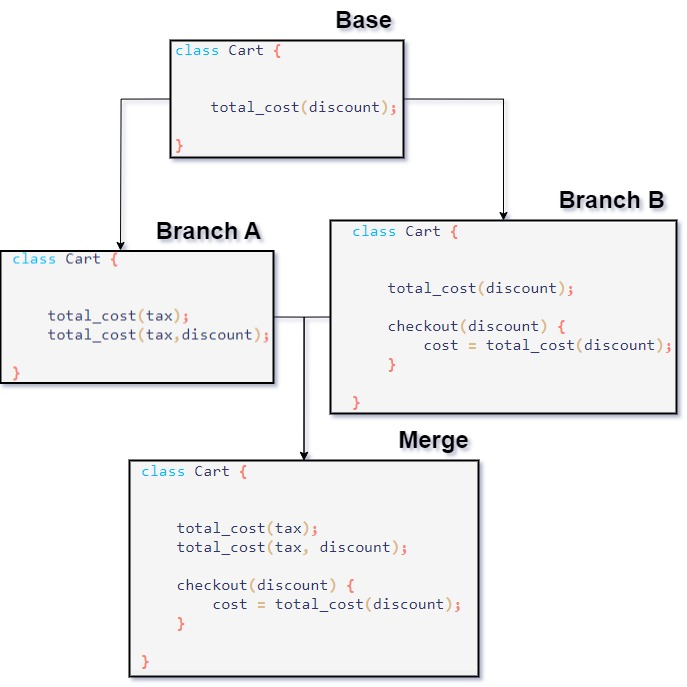
\includegraphics[width=0.86\textwidth]{conflict}
    \caption{Model of the motivating example conflict, with Base, Branch A, Branch B and Merge versions of the code.}
    \label{fig:conflict}
\end{figure}

\section{Goal} \label{sec:goal}

The goal of this research project is to assess to what extent existing Large Language Models can be used to identify semantic conflicts, both textually and through the generation
of appropriate unit tests. By comparing our results to existing prompts for unit test generation, we will assess to what extent, if any, we improved on and how to further develop
unit test generation for semantic conflicts using LLMs.
\todo{review}
\section{Study} \label{sec:study}

Following an initial exploratory phase, where different prompts, techniques and models were experimented with, our work approaches the issue by answering
3 research questions:

1. To what extent can a LLM textually explain a semantic conflict present in a merge.

2. To what extent can a LLM generate appropriate unit tests, given a textual explanation of the semantic conflict. 

3. To what extent do existing prompts generate appropriate unit tests and how do they compare to the prompt we developed. 
\todo{review}

\section{Thesis Structure} \label{sec:struct}


\Cref{chap:intro} introduces the topic and problem at hand.
\Cref{chap:rw} details existing related work on the topics at hand.
\Cref{chap:study} described our study and research questions and \Cref{chap:results} answers each research question.
\Cref{chap:conclusion} gives a conclusion.

\chapter{Related Work} \label{chap:rw}

The following sections introduces the two main topics dealt with in this dissertation (merge conflicts and the usage of large language models for software verification and test generation). They explore related work and how we can build on it to develop our approach.

\section{Semantic Conflict Detection}

The study of merge techniques and conflicts has a long history, likely even predating the specific terminology itself. Thus there is a large corpus of work to explore

Several related works exist which seeks to develop methods that can more systemically identify adulterated behaviour arising from semantic conflicts.

\subsection{Detection without Testing}

Several solutions exists which attempt to identify the presence of semantic conflicts without generating unit tests. An example of this rests on verifying overriding assignment: if a merge was successful where the same variable was assigned in both A and B, it's likely this is unintentional and there is a conflict. Thus, the solution checks if such a situation happens and reports if so to the developers~\cite{kn:assigne}.


Static analysis solutions have been considered, implementing the previous overriding assignment checks, inter procedural data flow and program dependence graph, which try to find data and control flows between the changes done by both developers, as well as confluence, which checks if there is data and control flows from both branches that flow into some common path. This static analysis shows much better F1 score and recall than dynamic analysis techniques, but much worse precision~\cite{kn:staticanal}.


The tool DeltaImpactFinder compares the impact of a change in the origin and destination branches, calculating the difference, the ``Delta-Impact''. To measure impact, dependencies are mapped out: the assumption is that when an entity is changed it's dependencies are impacted. A semantic conflict is identified if there are missing or extra dependencies and this can be identified with the calculation of the delta-impact~\cite{kn:deltaimpact}.

The notion of semantic conflict-freedom is seen as a sufficient condition for correctness. The SafeMerge~\cite{kn:safemerge} tool seeks to verify the presence of semantic conflict-freedom in the merge process, avoiding the creation of semantic conflicts. Semantic conflict-freedom can be defined, for branches O (Origin), A, B and M (Merge), for all i inputs:
\begin{itemize}
  \item If out(O,i) $\neq$ out(A,i), then out(M,i) = out(A,i)
  \item If out(O,i) $\neq$ out(B,i), then out(M,i) = out(B,i)
  \item Otherwise out(O,i) = out(A,i) = out(B,i) = out(M,i)
\end{itemize}

\subsection{Generation of Unit Tests}

In identifying the presence of semantic conflicts in a merge conflict, developed solutions have focused on the automatic generation of unit tests.

By Da Silva et al, we find an attempt at identifying cases of semantic conflict by applying automated behaviour change detection~\cite{kn:leuson}. In summary, with a base commit B, a left L, right R and merge M, they observe that a generated unit test that passes in L but fails in B partially reveals the effect of the changes made in that branch. If the test then fails in M, it is likely the changes made in R interfere. To generate unit tests they used EvoSuite~\cite{kn:evosuite} and Randoop~\cite{kn:randoop}.

In their analysis they found that the developed tool only detected interference in four out of 15 changes within merge scenarios that do actually suffer from interference, corresponding then to a recall of 0.267. While this is a very modest rate, it displayed no false positives (precision of 1) and thus could likely be integrated in a testing process to prune possible merge conflicts early, or further studied and refined.

 Building upon their previous work, \citet{kn:leuson2} proposed SAM (SemAntic Merge), a tool that generates tests upon merges in Java. It can be found at \url{https://github.com/leusonmario/SAM}. In summary, SAM initially does a simple textual merge to integrate the difference branches while identifying possible textual conflicts. After merging four program versions are built, to fully describe the merge scenario under test: Base, Left, Right, Merge. Source code transformations to improve testability are also part of the process, but optional. Finally, the test generation tools are fed objects serialized during the execution of existing test suites. After applying four test generations tools: EvoSuite~\cite{kn:evosuite}, Differential EvoSuite, Randoop ~\cite{kn:randoop} and Randoop Clean, their own adapted version of Randoop, SAM executes the generated tests against the four versions of the program, identifies which tests failed, interpreting it with pre-defined interference criteria heuristics and from there reports conflicts, if detected ~\cite{kn:leuson2}.

Detecting nine out of 28 conflicts, it shows improvements over previous work: the authors specifically highlight the best performance when combining tests from only EvoSuite and Differential EvoSuite. Regarding behaviour changes specifically, 89 are found. 
In both cases, they highlight the ability of transformations (for example, making private fields public) to increase testability, showing moderate improvements in some tested scenarios, with 20 additional changes being detected and three additional conflicts detected (Differential Evosuite detects 3, each other generator detect one conflict each).  Regarding the 19 false-negatives, 11 of them showed behaviour changes, which were not caused by the changes due to the semantic conflicts~\cite{kn:leuson2}.


\citet{kn:nuno} has proposed the tool UNSETTLE (aUtomatic uNit teSt gEneraTion for semanTic confLict dEtection). This tool, which can be found at \url{https://github.com/conflito/unsettle}, is composed of two modules:

Changes-Matcher identifies the possible presence of semantic conflicts, by first computing the changes between different versions (base and variants) and then comparing it to a set of patterns (listed in \Cref{table:pattern-table} describing common sources of conflicts as a base. From this it generates a DSL file, highlighting which methods and classes should be put under test to identify the conflict.

The second module is the test generator, a modified version of EvoSuite that takes the previously created artifact as an input to guide test generation.

Of particular interest to us is Changes-Matcher, as this is also the starting point for our work, with the usage of a LLM over EvoSuite for test generation instead.

\begin{table}[t]
\setlength\extrarowheight{2pt}
\begin{tabularx}{\textwidth}{llX}
 \toprule
 \textbf{Group} & \textbf{ID} & \textbf{Description} \\
 \midrule
 Change Method  & CM & Update two different dependencies of a method or update one method and concurrently update one of its
dependencies \\ 
 \hline
 Change Method
and Field & CMF & Change the type of one field to a type that does not
override a method while a dependency for the method
is added to a method that reads the field
 \\
 \hline
 Dependency
Based & DB & Update a method while a dependency to it is added
concurrently \\
 \hline
 Field Hiding & FH & Hide the field of a superclass in a subclass and concurrently add a method in the subclass that writes the
super field
 \\
 \hline
 Overload by Access Change & OAC & Change the visibility of an overloaded method and
concurrently add a dependency to it \\ 
 \hline
 Overload by Addition & OA & Overload a method and concurrently add a dependency to it \\  
 \hline
 Parallel Changes & P & Concurrent changes to the same entity, i.e., method
(PM), constructor, (PC) or field (PF) \\ 
 \hline
 Remove Overriding & RO & Remove the override of a method and concurrently
add a dependency to it \\  
  \hline
 Unexpected Overriding & UO & Override a method in a subclass while a dependency to it is added concurrently (AO) or override an
Object-inherited method and concurrently add a dependency to it (UO) \\
 \bottomrule
\end{tabularx}
\caption{\label{table:pattern-table}Semantic Conflict Patterns identified by Changes-Matcher~\cite{kn:nuno}.}
\end{table}


Ti Jao et al have proposed test oracles for program merges. Most significantly, not only do they support two and three way merges but also octopus merges. The developed tool, TOM (testing on merges), generates tests to identify unexpected and lost behaviour. For this, they implement diff-line as a criteria, guiding the tests to cover lines that have been modified between the different program versions, generating different assertions for different versions. Stability checking is done: the test is rerun five times before being handed to the developers. The tool identifies 45 three-way and 87 octopus merges, from a universe of 389 of each~\cite{kn:ji2022}.

\Cref{table:tool-comparison} shows a comparison between some key features of the presented solutions.


\begin{table}[t]
\setlength\extrarowheight{2pt}
\begin{tabularx}{\textwidth}{p{0.15\textwidth}p{0.17\textwidth}p{0.10\textwidth}p{0.13\textwidth}p{0.305\textwidth}}
  \toprule
  \textbf{Tool} & \textbf{Recall} & \textbf{Octopus Merge Support} & \textbf{Publicly Available} & \textbf{Test Generator} \\
  \midrule
  SAM & 43\% \newline (12 out of 28) & No & Yes & EvoSuite, Differential EvoSuite, Randoop, Randoop Clean \\ \hline
  UNSETTLE & 35\% \newline (6 out of 17) & No & Yes & EvoSuite \\ \hline
  TOM & 17\% \newline (132 out of 778) & Yes & No & EvoSuite \\
 \bottomrule
\end{tabularx}
\caption{\label{table:tool-comparison}Comparison of SAM~\cite{kn:leuson2}, UNSETTLE~\cite{kn:nuno}, and TOM tools~\cite{kn:ji2022}.}
\end{table}


% 12 out of 28 SAM
% 132 out of 778 TOM
% changes matcher always finds it, tests are 6 out of 17

\section{Test Generation}

\subsection{Traditional Automatic Test Generation}

Traditional methods of automated test generation can be divided into random and search-based techniques. The former, being random, is simpler and faster, while the latter employs heuristics and search algorithms to fulfill some criteria, like maximizing code coverage.

Randoop is one such example of random test generation. Some of the disadvantages of this technique can be mitigated with the employment of feedback-direction~\cite{kn:randoop}. Effectively, the search space of possible random tests is pruned, by guiding the test generator towards valid cases, avoiding expansion on invalid test cases~\cite{kn:randoop}.

EvoSuite implements search-based automatic test generation for Java code, aiming for tests that achieve high coverage, while being as small as possible and providing assertions. To achieve this they implement both evolutionary search to evolve the suite with respect to a coverage criterion and mutation testing to generate assertions~\cite{kn:evosuite}.

EvoSuiteR extends EvoSuite, aiming to provide automated generation of regression tests. Thus it takes account two versions of the software and aside from coverage, it considers state distance (``how different is the state of
all objects in the test suite across the two versions'') and control flow distance (``how
far are the two versions from diverging'')~\cite{kn:evosuiter}.

The symbolic execution technique, while introduced in the 70s has been more explored as computing power increased. It executes programs with symbolic rather than concrete values: assignments are represented as functions and conditionals as constraints. From this, we can identify specific paths and branches. This can be done statically, we symbolic execution techniques first used to derive all paths or dynamically, with symbolic execution being updated throughout execution, allowing us to find alternatives to the current branch~\cite{kn:symbolicexec}.


Similar suites have been developed, for example, for Python~\cite{kn:pynguin}.

\subsection{Test Generation with LLMs}

The recent explosion in complexity and popularity of LLMs has suscitated developer interest in their abilities with regards to accelerate and automate software engineering. Angela Fan et al identified that by 2023 3\% of pre-prints were related to Large Language Models and 11\% of those related to their use in software engineering~\cite{kn:angela}. Particularly relevant is their ability to generate tests, with an expectation that they could achieve better coverage, correctness and readability than previous techniques of automated test generation~\cite{kn:junjiewang}.
In comparison to traditional suites for automated test generation, such as EvoSuite, Palus, Randoop, and JTExpert, ChatGPT has shown, given right tuning of temperature settings, to evidentiate equivalent robustness~\cite{kn:gptunitbra}.
From surveys done on the topic, we find Codex and GPT variants to be the most commonly used LLMs for this issue~\cite{kn:junjiewang}.

While many studies suggest LLMs are competitive with traditional methods of software generation, we can also find evidence to the contrary. Specifically, testing across several LLMs, including Codex, StarCoder and GPT-3.5-Turbo, shows they fail in all regards compared to EvoSuite, primarily due to the generation of non-compilable code, often due to ``hallucination'' of non-existent types and methods~\cite{kn:siddiq2023empirical}. Yutian Tang and others find EvoSuite outperforms ChatGPT in code coverage~\cite{kn:tang2023chatgpt}. Given the novelty of the technology, it is unsurprising there is such variance in reported results and research, but it is worth investigating. Research on Copilot, Github's solution based on Codex, show interesting results: while 92.45\% of tests generated without an existing testing suite either failed, were broken or empty, by providing an existing suite the figure would drop to 54.72\%~\cite{kn:githubcopilot}, suggesting that providing this information and a structure to work off is extremely valuable, despite still wielding extremely high failure rates.

Despite variable conclusions regarding correctness and coverage, it seems generally agreed that ChatGPT is good at generating readable code. Yutian Tang et al highlight that despite minor style errors, primarily in identation, the generated code is clear and easy to understand~\cite{kn:tang2023chatgpt}. A survey of software developers has found ChatGPT to have comparable and even better readability than manually written tests~\cite{kn:chattester}.


Given the LLM can produce unreliable results, the maximization of ChatGPT's abilities with regards to test generation has been explored: techniques such as prompting the LLM for a explanation of what the code is intending to do~\cite{kn:nuances} and feeding error messages from codes that fail to compile or execute as intended back to the LLM for correction~\cite{kn:chattester} have shown an amazing capacity for test generation, given the right prompting.

Regarding prompting, understanding how to best engineer prompts to achieve the desired output from the LLM is a particularly relevant issue. For example, in the generation of test inputs, research found ``generate diverse test input'' to be preferable over ``generate test inputs that result in different outputs between PUT and reference versions'', as ChatGPT could not accurately identify the nuances required to correctly carry out the latter's instructions~\cite{kn:nuances}.
With unit testing generation in particular, Zhiqiang Yuan et al, in developing the ChatTester tool, highlight the importance of combining a natural language descriptor with the appropriate code context~\cite{kn:chattester}.

\begin{prompt}
public class Travis {
public static final String TRAVIS NAME = ""travis-ci"";
public static final String TRAVIS = ""TRAVIS"";
public static final String TRAVIS JOB_ID = \"TRAVIS_JOB_ID\";
public static final String TRAVIS PULL_REQUEST = \"TRAVIS_PULL_REQUEST\";
public Travis (final Map<String,String> env);
public boolean isSelected();
public String getName();
public String getJobId();
public String getBranch();
public String getPull Request();

//Focal Method
public Properties getEnvironment() {
  Properties environment new Properties();
  addProperty (environment, ""travis_job_id"", getProperty (TRAVIS_JOB_ID));
  addProperty (environment, "travis_pull request", getProperty(TRAVIS PULL REQUEST));
  return environment;
  }
}

You are a professional who writes Java test methods;
Please write a test method for the method "getEnvironment()" based on the given information using Junit4.
\end{prompt}

Another technique utilised is asking the LLM to infer the intention before developing the tests, which leads it to generate correct tests where basic prompting would fail~\cite{kn:chattester}.

\begin{prompt}
Intention Prompt for ChatGPT

// Focal class
public class StrBuilder {
  public StrBuilder();

  // Focal method
  public StrBuilder setCharAt(final int index, final char c){
    if(index < 0 || index >=length()) {
      throw new StringIndexOutOfBoundsException(index);
    }
    buffer[index] = ch; return this;
  }
}

Please infer the intention of the "setCharAt(final int, final char)".
\end{prompt}

\begin{response}
The intention of 'setCharAt(final int index, final char c)' in the 'StrBuilder' class is to set the character at the specified index in the character buffer to the given character.
\end{response}

\begin{prompt}
Generation Prompt for ChatGPT

// Method Intention
The intention of 'setCharAt(final int index, final char c)' in the 'StrBuilder' class is to set the character at the specified index in the character buffer to the given character.

You are a professional who writes Java test methods.
Please write a test method for the "setCharAt(final int, final char)" with the given Method intention.
\end{prompt}

While they argue that it is little known how effective these strategies are, \citet{kn:johnny} and others highlight several prompting strategies: give examples of desired interaction, write prompts that look somewhat like code and repeat yourself. They note difficulties participants have in prompt generation, such as avoiding giving examples due to fear the LLM will simply replicate it, difficulty in searching online for help and adapting existing solutions and overgeneralizing from a single example~\cite{kn:johnny}.

In prompting we can distinguish a few types of prompts: zero-shot, where instructions are simply given, few-shot, where examples of inputs and outputs are given and few-shot with preamble, combining the previous two examples to give both a preamble instructing the LLM on what to achieve, follow by examples of inputs and outputs~\cite{kn:promptprofiannaca}

Given the natural language aspect of LLM prompting is one the features that most distinguishes it from classical programming, it is worth exploring methods of systematizing it, making it work more like code. It is with this objective that LMQL (Language Model Query Language) was developed, introducing a scripting based query language~\cite{kn:lmql}. Evidence shows it reduces computing costs by up to 80\%~\cite{kn:lmql}.

The team behind ChatUniTest presents a two step prompting system, where instructions of what is to be done and how are first provided~\cite{kn:chatunitest}:

\begin{prompt}
Setup Prompt
Please help me generate a JUnit test for a specific Java method using JUnit5 and Mockito3.
I will provide the source code for the method, relevant method signatures and fields, required dependencies, Java class containing the method, expected behaviour, and involved classes in the project.
Create a test that imports necessary dependencies, compiles without errors, and achieves maximum branch and line coverage. 
No explanations needed. 

Specific Test Information
The focal method is ... in the class ..., and the class information is .... The brief information of involved class ... is ...   
\end{prompt}


The training of LLMs in open source repositories gives cause to the fear that automatic test generation might be reliant on the model being trained in the code under test, or simply replicating existing testing suites. To assuage this, it was identified that even when generating tests for packages hosted in GitLab (which were not used to train the LLM under study, gpt3.5-turbo), they still maintained high coverage. In addition, it was found that 60.0\% of the tests had <= 40\% similarity to existing tests and 92.8\% had <= 50\%. Thus we can conclude the LLM is not simply copying tests from the training set without alteration~\cite{kn:max}.


\section{Summary}

The related work aids our own work in several ways: the work explored as regards unit test generation can provide show us a baseline functioning of the idea we are trying to implement. Particularly, we can use their statistics regarding percentage of conflicts found to assess whether our own solution is an improvement with regards to previous work.

Crucially important too is the work of \citet{kn:nuno} and, as previously mentioned, the developed Changes-Matcher.

The study of works on LLM test generation should also prove useful in the future, allowing us to get a better understanding of their functioning and capabilities, as well as providing ideas and prompt generation techniques which we may have to apply in the future.

\chapter{Empirical study}\label{chap:study}

This chapter describes the study conducted to assess the capabilities of LLMs
(in particular, ChatGPT and GitHub Copilot) at identifying, explaining,
and revealing semantic conflicts in merge commits.
% This chapter is divided into two phases: an initial exploratory phase, where an unstructured exploration allowed us to develop prompts, identify characteristics of the LLM and narrow down on its abilities and limitations.  In a second phase, work was systematized, with the elaboration of research questions and metrics to evaluate results.

\section{Experimental subjects}\label{chap:study:subjects}

\begin{table}[t]
\centering
% \tabcolsep=1cm
% \renewcommand{\arraystretch}{0.90}
\begin{tabular}{@{\extracolsep{\fill}} lll} \toprule
                 & Real Conflict & Type of Conflict \\
\midrule
Point            & No  & Change Method \\
Fabricated (RO)  & No  & Remove Override \\
Fabricated (OAC) & No  & Overload by Access Change \\
Cart (PF)        & No  & Parallel Field \\
Cart (PM)        & No  & Parallel Method \\
Cart (CM)        & No  & Change Method \\
Antlr            & Yes & Parallel Field \\
OkHttp           & Yes & Parallel Method \\
Retrofit         & Yes & Parallel and Change Method \\
\bottomrule
\end{tabular}
\caption{Subjects used in the empirical study, with information on whether subject is fabricated or extracted from a real software project, as well as the type of conflict found.\label{tab:subjects}}
\end{table}

% To assess the validity of a developed solution, a collection of subjects to test must be collected.
Previous works have established catalogs of merge commits with semantic conflicts
to ease the evaluation and comparision of any developed solution.

\citet{kn:safemerge} \todo{describe it.  how many conflicts are there, where they
come from, what type, etc.}
% analyze popular repositories, i.e., Elasticsearch, libGDX, iosched, kotlin, MPAndroidChart, okhttp, retrofit, RxJava, and the Spring Boot framework, where they find 11 positive results \todo{the results dont really matter in this subsection}.

\citet{kn:leuson} \todo{describe it.  how many conflicts are there, where they
come from, what type, etc.}

\citet{kn:nuno} \todo{describe it.  how many conflicts are there, where they
come from, what type, etc.}

\citet{kn:leuson2} established 28 merge commits with conflicts, from a total of 85.   \todo{describe it.  how many conflicts are there, where they come from, what type, etc.}

For our study we elected the subjects used in \citet{kn:nuno}'s study.  It is
publicly available, closely related to our own work, and also allowing us to
draw direct comparisons.  Most importantly, it aggregates merge instances from
both \citet{kn:leuson} and \citet{kn:safemerge}, while also providing valuable
information, due to the work developed, such as the specific type of conflict
present and whether it was detected and correctly tested by UNSETTLE~\cite{kn:nuno}
(providing us with a ``base truth'').  Furthermore, it has compiled a set of
fabricated conflicts, which provide simpler isolated examples that can aid us as
they should be easier to identify, explain, and reveal.

While analyzing \citet{kn:nuno}'s set, we found the predominant types of semantic
conflicts in real scenarios where ``Parallel Changes in Field'', ``Parallel Changes in Method'',
and ``Change Method''.  Using a simple Cart class as a base, three examples were
made for these scenarios.  These Cart examples were part of the group of subjects used to answer and evaluate the research questions we defined.  These were complemented by a simple Point class, two examples fabricated by Castanho of type ``Override by Access Change'' and ``Remove Override'', %which had achieved good results in exploratory testing\todo{not clear.  perhaps to early to say this}, 
Antlr4, OkHttp and Retrofit, respectively a simple and two hard to test real-world scenarios.
The collection of subjects and corresponding type of conflict can be found in \Cref{tab:subjects}.

% It is worth examining each subject and it's corresponding conflict, to make understanding the results easier.

\subsection{Point}

\subsubsection{Conflict Type: Change Method}

Point consists of a simple class for a two dimensional point, with fields \texttt{x} and \texttt{Y}.
Other than getters and setters, it's most relevant methods are \texttt{move} and \texttt{distance}.
Originally, the method \texttt{move} increments both \texttt{x} and \texttt{y} by 1, while \texttt{distance} computes the euclidean distance to \texttt{(0,0)}.
In branches A and B, \texttt{move} is modified to increment by \texttt{distance} while \texttt{distance} is modified to compute
the manhattan distance.  The conflict then arises when code is merged.  \texttt{move} was modified with the expectation that it would move
based on the euclidan distance, but with the merging of the other branch it will move differently.

\subsection{Fabricated}

The Fabricated subject revolves around events: ticketing, scheduling, installations, etc. The two
conflicts that make the two subjects relate to different parts of the code.

\subsubsection{Conflict Type: Remove Override}

The classes involved in the conflict are \texttt{Instalacao} and \texttt{InstalacaoAssentos}, which extends the former.
Of is the method \texttt{helpString}, which returns a string with class information.  This method is present
in both classes with different implementations (thus \texttt{InstalacaoAssentos} overrides it). In branch A,
\texttt{hashString} is introduced in \texttt{InstalacaoAssentos}: it takes \texttt{helpString} and hashes it. In branch B,
the \texttt{helpString} from \texttt{InstalacaoAssentos} is deleted. Thus, the conflict arises because in the merge,
\texttt{hashString} will be calling the \texttt{helpString} from \texttt{Instalacao} and the has values returned will be different.

\subsubsection{Conflict Type: Overload By Access Change}

The classes involved are \texttt{Event} and \texttt{Producer}, where the former has a ManyToOne relationship with the latter.
In \texttt{Producer}, there are two methods: \texttt{setResgistration(Integer)} and \texttt{setResgistration(int)}. The former sets
the producer's \texttt{registrationNumber} to the \texttt{intValue()} of the \texttt{Integer + 10}. The latter just sets the given value.
In branch A, the \texttt{int} version of the method is made private. In branch B, a \texttt{setProducerNumber(int)} function is added
to \texttt{Event}: it checks if the \texttt{Producer} is null and if not, calls \texttt{setResgistration} with the given value. In B, this will
call the \texttt{int} version of the method, as it is still public, but after the merge, the \texttt{Integer} version will be used instead,
hence the conflict.

\subsection{Cart}

Cart consists of a simple class representing a shopping cart, with auxiliary classes for users and items.
Its fields correspond to a dictionary of discounts, with string associated to doubles, a list of items in the cart
and the associated user.
It has the appropriate methods to add items to the cart, calculate the cart value, and checkout with a given discount code,
subtracting the value from the user's balance.
Cart has some pecularities which may differ from real-world classes of the same type. These include the fact that checkout
requires a discont code as an argument (there is no checkout without discount) and that items can only be added one by one, without
any way to add a collection all at once.  Notably their auxiliary classes contained only public fields, with no getters and setters, as
well as lacking expected fields such as String type ``name'' fields. These divergences from the norm came to matter when it came to
test generation.

\subsubsection{Conflict Type: Parallel Field}

The base of this conflict has some alterations compared to the other Cart versions: a more full dictionary of discounts,
a method to get the key set and a boolean method (\texttt{checkForDiscountRenewal}) that returns \texttt{true} or \texttt{false} whether the key set is less or equal than six.
The changes correspond to the removal of a discount in the first line of the field, in branch A, and the removal of a discount in the last line, on branch B.
These merge correctly but emergent behaviour arises: the key set in merge is different from both the one in A and B.
The boolean method further makes this evident.

\subsubsection{Conflict Type: Parallel Method}

The changes relate to the sum\_items() method. At the start, it just goes trough the items in the list and sums together. In branch A,
a check that certified the return is greater or equal to 0 is removed. In branch B, the boolean coupon is added to item and if an item
is of type coupon, its value is removed rather than added. There is emergent behaviour in the merge, as coupons now allow carts of negative
value to exist.

\subsubsection{Conflict Type: Change Method}

The conflict arises due to the handling of checkout. In branch A, a check is added where if a user is of type admin,
\texttt{total\_cost} method returns 0. In branch B, a check is added in the \texttt{checkout} method: if \texttt{total\_cost} is 0, a runtime exception is thrown.
Naturally these changes conflict in the merge.

\subsection{Antlr}

\subsubsection{Conflict Type: Parallel Field}

Antlr is much like Cart (Parallel Field), but with additions instead of removals: it contains a String array called \texttt{python2Keywords}, which is returned as a set by the \texttt{getBadWords} method.
In branch A, the string ``del'' is added and in branch B, the string ``return'' is added.
Thus in the merged version we will have a emergent version of the \texttt{BadWords}
set, with different length and contents compared to both previous versions.

\subsection{OkHttp}

\subsubsection{Conflict Type: Parallel Method}

OkHttp provides an HTTP client. The class OkHttpClient configures and creates HTTP connections. This process involves
the \texttt{copyWithDefaults} method, which creates a shallow copy, using system defaults for fields which are not set. Both branches
modify this method, one by changing how \texttt{failedRoutes} are handled and adding a field for transports, while the other replaces
the default hostname verifier with a custom implementation, \texttt{OkHostnameVerifier}. As a result, the copy returned on merge will
be different from both branches, and this difference will trickle down into the initialization of \texttt{HttpURLConnectionImpl}, which
as the copy as an argument.

\subsection{Retrofit}

\subsubsection{Conflict Type: Parallel and Change Method}

Another HTTP client. Relevant to the conflict is the class \texttt{RequestBuilder}, which builds HTTP requests from Java method invocations. The methods modified
in the conflict are \texttt{build}, which returns a \texttt{Request}, and the method \texttt{buildRelativeUrl}, which is invoked inside of \texttt{build}.
Branch A only modified how request queries are handled, by adding the appropriate \texttt{?} to the url when one is present.
Branch B adds several checks for null arguments for request query arguments, path parameters, form fields and multipart parts, throwing an exception or ignoring them as adequate.
Both of these chances are integrated and as a result, the behaviour of the construction of a \texttt{Request} is different in the merge.

\section{Large Language Models (LLMs)}

While preliminary work sought to explore ChatGPT~\cite{kn:gpt} and Llama~\cite{kn:llama} (both CodeLlama and Llama 2), hardware constraints, particularly limited GPU RAM in the machines at our disposal, meant we were unable to explore Llama.  Bing AI~\cite{kn:bingAI} and Bard~\cite{kn:bard} were also considered, but they were problematic due to very stringent message size limits, in the case of Bard, and generally worse results: Bing AI, for example, could not wait for all the information to be sent, if split in more than one message and thus generated confused responses. ChatGPT, being hosted online for free and with generous message size limits, proved to be the most reliable option. Despite this, many capabalities that could prove invaluable for this work remained locked behind a premium paywall.
The instance of ChatGPT used was the web-based ChatGPT 3.5 Turbo, with default temperature, during the first semester of 2024.
The version of GitHub Copilot was version 1.5.6.5692.

\section{Research questions}

\begin{itemize}
  \item[\textbf{RQ1:}] Can ChatGPT identify, understand, and explain, whether
  there is a semantic conflict in a merge commit?

  \item[\textbf{RQ2:}] Given an explanation of a semantic conflict in a merge
  commit, can ChatGPT generate unit test case that are able to identify it?
  % the emergent behaviour of to a semantic conflict, if given an explanation of it?

  \item[\textbf{RQ3:}] Can state-of-the-art prompts lead ChatGPT to generate to
  unit test cases that are able to identify semantic conflicts?  How do they
  compare to the prompt used in RQ2?
\end{itemize}

\section{Experimental procedure and metrics}

\subsection{RQ1}

In our first research question we established sought to more systematically evaluate ChatGPT's capabilities to assess and describe semantic conflicts.
We first settled on a prompt, based on the prompts that were iteratively developed on previously work.

\begin{prompt}
You are a software developer that has to assess whether there is a semantic conflict in a merge commit.  Given the base version of the class, the diff from base to a version A, the diff from base to a version B and the merged version of the class, assess whether there is a semantic conflict and explain it.

Base version:
```java
```

Diff version A and the base:
```diff
```

Diff version B and the base:
```diff
```

Merge version:
```java
```
\end{prompt}

% For each semantic conflict example, as listed previously,
The prompt was submitted three times to account for the randomess nature of the
LLM, which in turn allowed us to see a broader range of responses and avoiding
what might be one-time flukes.

As an example how one would instantiate this prompt is listed below for the
Point subject, where a conflict is introduced by the simultaneous change of
euclidean to manhattan distance followed by the usage of the same distance method
in another method.
\begin{prompt}
You are a software developer that has to assess whether there is a semantic conflict in a merge commit.  Given the base version of the class, the diff from base to a version A, the diff from base to a version B and the merged version of the class, assess whether there is a semantic conflict and explain it.

Base version:
```java
public class Point {
    private double x;
    private double y;

    public Point(double x, double y) {
        this.x = x;
        this.y = y;
    }

    public double getX() {
        return x;
    }

    public double getY() {
        return y;
    }

      public void move() {
          this.x += 1;
          this.y += 1;
      }

    public double distance() {
        return Math.sqrt(Math.pow(getX(), 2)+ Math.pow(getY(), 2));
    }

    public String toString() {
        return "(" + getX() + ", " + getY() + ")";
    }
}
```

Diff version A and the base:
```diff
@@ -16,8 +16,9 @@ public class Point {
      }

      public void move() {
-         this.x += 1;
-         this.y += 1;
+         double dist = distance();
+         this.x += dist;
+         this.y += dist;
      }

      public double distance() {
```

Diff version B and the base:
```diff
@@ -21,7 +21,7 @@ public class Point {
      }

      public double distance() {
-        return Math.sqrt(Math.pow(getX(), 2)+ Math.pow(getY(), 2));
+        return Math.abs(getX())+Math.abs(getY());
      }

      public String toString() {
```

Merge version:
```java
public class Point {
    private double x;
    private double y;

    public Point(double x, double y) {
        this.x = x;
        this.y = y;
    }

    public double getX() {
        return x;
    }

    public double getY() {
        return y;
    }

      public void move() {
          double dist = distance();
          this.x += dist;
          this.y += dist;
      }

    public double distance() {
        return Math.abs(getX())+Math.abs(getY());
    }

    public String toString() {
        return "(" + getX() + ", " + getY() + ")";
    }
}
```
\end{prompt}
%
% \todo{Jose: Given the motivational example is one of the subject, I might not
% sure we should provide results in here.}
% This prompt nets us the following response from the LLM.
%
% \begin{response}
% To assess whether there is a semantic conflict in the merge commit, let's analyze the changes introduced in versions A and B compared to the base version, and then compare them with the merged version.
%
% ### Changes introduced in Version A:
% - The `move()` method has been modified to calculate the distance using the `distance()` method and then update the `x` and `y` coordinates accordingly.
% - This change effectively moves the point by the distance it currently is from the origin.
%
% ### Changes introduced in Version B:
% - The `distance()` method has been modified to calculate the Manhattan distance instead of the Euclidean distance.
% - The Manhattan distance is calculated by taking the absolute value of the x and y differences.
%
% ### Analysis of Merged Version:
% - The `move()` method from Version A has been kept in the merged version, which calculates the distance using the Euclidean distance.
% - The `distance()` method from Version B has been kept, which calculates the Manhattan distance.
%
% ### Potential Semantic Conflict:
% - The potential conflict arises from the inconsistency between how distance is calculated in the `move()` method and the `distance()` method in the merged version.
% - While the `move()` method assumes Euclidean distance for movement, the `distance()` method calculates the Manhattan distance.
% - This inconsistency could lead to unexpected behavior, as the `move()` method might not accurately reflect the intended behavior of the `distance()` method.
%
% ### Conclusion:
% - There is a semantic conflict in the merge commit because the merged version contains methods with conflicting assumptions about how distance should be calculated.
% - Resolving this conflict would require ensuring consistency in the distance calculation method used throughout the class, either sticking with Euclidean distance or Manhattan distance for both `move()` and `distance()` methods.
% \end{response}

To evaluate the answers generated by ChatGPT, we established five metrics (A--E), each with likert scales.
%
\begin{itemize}
  \item[\textbf{A}:] Changes between branches correctly identified (Correct description of Version A and B).
  \begin{itemize}
    \item[\textbf{0}:] Large errors in description for both branches.
    \item[\textbf{1}:] Large error in description of one branch.
    \item[\textbf{2}:] Minor insignificant errors.
    \item[\textbf{3}:] Changes correctly identified.
  \end{itemize}

  \item[\textbf{B}:] No conflict misunderstanding (Does not describe textual conflict, understand merge succeed).
  \begin{itemize}
    \item[\textbf{0}:] Understands conflict as textual.
    \item[\textbf{1}:] Understands the conflict as semantic.
  \end{itemize}

  \item[\textbf{C}:] Positive response (3 types: says conflict exists/may exist/does not exist)
  \begin{itemize}
    \item[\textbf{0}:] Denies existence of conflict
    \item[\textbf{1}:] Asserts conflict is possible
    \item[\textbf{2}:] Asserts conflict exists
  \end{itemize}

  \item[\textbf{D}:] Origin of conflict described (What code interactions lead to altered behaviour)
  \begin{itemize}
    \item[\textbf{0}:] Incorrect or non-existent explanation
    \item[\textbf{1}:] Identifies origin of conflict, with lack of clarity or imprecisions
    \item[\textbf{2}:] Identifies origin of conflict, with lack of confidence
    \item[\textbf{3}:] Identifies origin of conflict
  \end{itemize}

  \item[\textbf{E}:] Effect of conflict described (What is the result of the code interactions/expected output)
  \begin{itemize}
    \item[\textbf{0}:] Result of conflict is omitted, too vague or wrong
    \item[\textbf{1}:] Result of conflict is expressed, but with imprecisions or generically
    \item[\textbf{2}:] Possible code outputs are expressed, with little confidence
    \item[\textbf{3}:] Assertively points out expected outputs due to conflict
  \end{itemize}
\end{itemize}

% From this we derive the metrics: A=3, B=1, C=2, D=3, and E=2.
% In this case, given the correctness of the answer, all metrics have perfect scores,
% except for metric D (Effect of conflict described), due to the reduced confidence.

\subsection{RQ2}

In this research question we sought to evaluate ChatGPT's test generation ability. Specifically, whether it could generate tests that would show the evidence the semantic conflict, given an explanation of the conflict.
For instance, taking the Point as an example, if ChatGPT generates a unit test that exercises the \texttt{move} method, we would identify the conflict by generating a test that passes in the merge but fails in branch A and branch B, corresponding to the definition of emergent behaviour (see \citet{kn:nuno}, Chapter 3.1 for more information).
In this case, the test run in the different versions would show us the altered behaviour of \texttt{move} due to the conflict.

It is known that the generation of incorrect code, whether semantically or syntatically incorrect is a frequent issue \todo{where?}. \Citet{kn:wheredofail} showed the extent to which this applies across a varied range of LLMs,
indicating this is a general issue and not specific to any individual model. As regards ChatGPT (and test generation) specifically, \Citet{kn:chattester} found that only 42.1\% of generated tests compiled and a further
24.8\% passed. Of those that did not pass, they failed because of faulty generation, not due to any preexisting bug in the code.
\Citet{kn:chattester} found the most common errors to involve symbol resolution, due to the usage of undeclared classes (which far overshadowed any other error), methods or variables. Other less frequent errors were accesses on private classes and the usage
of invalid types for operations, constructor or method parameters.
Errors during execution mainly fell on assertion errors, with a minor amount of runtime exceptions.

Taking this into account, to evaluate the tests we generated, corrections were made. These involved the smallest possible corrections to make the code compile and pass in merge, by correcting syntatic errors and failing asserts.
For example, given the following generated test:
\begin{response}
@Test
public void testSetProducerNumber() {
    Event event = new Event();
    Producer producer = new Producer();
    producer.setRegistrationNumber(123); // Set registration number
    event.setProducer(producer);
    int expected = 123;
    int result = event.setProducerNumber(456); // Try to set different registration number
    assertEquals(expected, result);
}
\end{response}
We applied the corrections and achieved this test:
\begin{response}
@Test
public void testSetProducerNumber() {
    Event event = new Event();
    Producer producer = new Producer();
    producer.setResgistrationNumber(123); // Set registration number
    event.setProducer(producer);
    int expected = 466;
    int result = event.setProducerNumber(456); // Try to set different registration number
    assertEquals(expected, result);
}
\end{response}
Here, we fixed a method call, which in correcting a typo in the code tried to call a non-existent function, and ammended the value to be used in the assertion.
Other common edits were ammending constructor calls with extra parameters or replacing getter calls for getters which did not exist with direct accesses.

From this we calculated the edit distance, which corresponds to the Levenshtein Distance, excluding comments.
In this case, it was four.

Where the test was incorrect to such an extent correction would require a major rework, corrections were not applied. This helped to distinguish logically sound tests
that suffered from minor easy-to-fix compilation errors from broken tests which were not useful for our purposes. Furthermore, these minor changes were liable to be automated,
either through scripting or through the usage of the LLM itself, as shown by \Citet{kn:chattester}.

We evaluated by observing whether a syntatically correct and passing unit test was generated and if not, the edit distance to a functioning version of one test. For failing tests, we also noted which error led to the failure of compilation or test. The types were:
\begin{itemize}
  \item Assert: The logic of the test makes sense, but the value of the assertion is incorrect.
  \item Constructor: The test fails to compile because an Object is incorrectly constructed.
  \item Branch: The test is functional, but does not make the conflict evident because it is testing for the wrong branch.
  \item Miss: Missing asserts, or existing assert does not target the conflict.
  \item Other: Assorted errors in test logic or method calls.
\end{itemize}
These allowed us to further evaluate how the prompting could be improved and if these errors could be fixed.

The basic structure of the prompt follows:
\begin{prompt}
You are a software developer that has to write a set of JUnit test cases to trigger a semantic conflict that has been identified in a merge commit.
Given the base version of the class, the diff from base to a version A, the diff from base to a version B and the merged version of the class, and an explanation of the existing semantic conflict, generate the appropriate JUnit test cases that trigger the conflict.

Base version:
```java
```

Diff version A and the base:
```diff
```

Diff version B and the base:
```diff
```

Merge version:
```java
```

Explanation of the semantic conflict:
Generate just code with necessary imports. No explanation needed.
\end{prompt}
Two versions of the prompt were run, each with three trials: in the first, the explanation was manually written, whereas in the highest performance answer from ChatGPT in RQ1 was used.
This way it could be evaluated to what extent this influence test generation results.

Testing of the subjects was done on the basis of identifying emergent behaviour: this involves the generation of unit tests that
pass in merge and fail in the parent branches (or one branch fails to compile)~\citep{kn:nuno}. This identifies the conflict by
asserting the behaviour present in merge that was not present before, ie, emerges.

\subsection{RQ3}

In this research question we sought to assess the relevance of our developed work by assessing the generative abilities of previous state-of-the-art prompts, which just generate tests for methods, with no conflict information.
We also used GitHub Copilot, which allowed us to consider to what extent the usage of another LLM affects test generation.

We selected four prompts:
\begin{itemize}
  \item Prompt \#1: From ``No More Manual Tests? Evaluating and Improving ChatGPT for Unit Test Generation'' by ~\citet{kn:chattester}.
  \item Prompt \#2: From ``Using Large Language Models to Generate JUnit Tests: An Empirical Study'' by ~\citet{kn:siddiq2023empirical}.
  \item Prompt \#3: From ``ChatUniTest: A Framework for LLM-Based Test Generation'' by~\citet{kn:chatunitest}.
  \item Prompt \#4: Second part of prompt 2, the test skeleton, but instead used GitHub Copilot for completion.
\end{itemize}
%
We then ran three trials were run for Prompt \#1 and Prompt \#3, whereas Prompt \#2 and \#4 only had one as they showed no variation (due to no temperature).
We evaluated the prompts in two steps: in a first step we observed if the generated tests compiled and in case they did, if the test generated were passing.
In a second step, we examined the test logic itself to see if the tests can potentially identify the semantic conflict, if the same type of simple corrections applied in RQ2 were applied.

\section{Threats to validity}

Based on the guidelines reported by \citet{wohlin2012experimentation}, we have
taken all reasonable steps to mitigate the effect of potential threats, which
are described in detail in this section.

\subsection{Threats to construct validity}

We recognize the threat to construct validity played by the prompts we developed, as it is possible they were not appropriate for the research questions
we defined. We mitigated this by exploring several techniques, both by studying state-of-art prompting techniques as well as experimenting with focus in our use case in particular, before settling on the prompts we defined, but other techniques might have yielded better
results.

\subsection{Threats to internal validity}

Internal validity may have influenced by human errors, such as minor errors in prompts or mistakes in the collection and computation of results.
We mitigated this with frequent internal revisions. % and several mistakes were caught.

\subsection{Threats to external validity}

A main threat to external validity was our reliance to the LLMs used, i.e., ChatGPT-3.5 Turbo and GitHub Copilot. While we made efforts to investigate other LLMs
we were constrained by hardware and financial limitations. Thus, these results are not necessarily generalizable and further study would be required to see how other models compare.  Nevertheless, these two are state-of-art solutions and existing research
does not seem to indicate any other existing LLM is significantly better.

    \chapter{Experimental results}\label{chap:results}

This chapters answers \textbf{RQ1 – RQ?}, which study \todo{???}.

\section{RQ1}\label{sec:results:rq1}

\begin{table}[t]
\centering
% \tabcolsep=1cm
% \renewcommand{\arraystretch}{0.90}
\begin{tabular}{@{\extracolsep{\fill}} lrrrrr} \toprule
                 & A - 3 & B - 1 & C - 2 & D - 3 & E - 3 \\
\midrule
Point            & 3.0 & 1.0 & 0.67 & 1.0 & 0.67 \\
Fabricated (RO)  & 3.0 & 1.0 & 1.0 & 2.0 & 0.67 \\
Fabricated (OAC) & 2.33 & 1.0 & 1.0 & 3.0 & 0.67 \\
Cart (CM)        & 3.0 & 1.0 & 1.0 & 1.67 & 0.67 \\
Cart (PF)        & 1.0 & 1.0 & 2.0 & 2.33 & 0.67 \\
Cart (PM)        & 3.0 & 1.0 & 0.67 & 2.0 & 2.0 \\
Antlr            & 1.67 & 1.0 & 0.0 & 0.0 & 0.0 \\
OkHttp           & 3.0 & 1.0 & 0.67 & 0.0 & 0.0 \\
\midrule
\textit{Average}  & 2.5 & 1.0 & 0.88 & 1.5 & 0.67 \\
\bottomrule
\end{tabular}
\caption{Average values per subject and metric.\label{tab:results:rq1}}
\end{table}

\Cref{tab:results:rq1} summarizes the metrics achieved per subject. From these we can note that:

A: ChatGPT is generally able to identify changes made between branches.

B: In none of our examples did the tool mistake the kind of conflict under discussion. This might be because the prompt did not assert the existence of a conflict, allowing negative responses, whereas other prompts, which asked to find a conflict that did exist, lead the model to find any explanation, which often consisted of describing a textual conflict.

C: Answers given tend to identify a conflict, but with uncertainty (with language such as "possible", "might"). In other cases, the cases where no conflict was found outweighed the cases where one was found with uncertainty.

D: Identification of the origins of conflict falls squarely in the middle of our given range.  When we exclude 0 value results, the average is 2.77 instead. This indicates to us in nearly half the cases, the model failed to produce any description, but when it did, it was generally very accurate.

E: ChatGPT struggles with accurately describing the results of semantic conflicts, ie, how the behaviour is specifically altered and how the outputs change. Indeed, even when the origin of the conflict is found, an accurate description of the results does not necessarily follow, with the topic being vague or not touched upon.

The complete prompts, with results and evaluated metrics, can be found in the attachments \todo{Which one? Do not forget to cref it here}.
\todo{how to ref? can ref html files or to put in body of text?}
An important observation to make is the variability of results, which highlights the importance of running 3 trials for our evaluation.
For example, the point class had high variation: two of the results failed to identify any conflict at all, but one of the three not only identified, but quite accurately describe it's origin and results.

In the more complex fabricated examples, the biggest issue was the identification of the effects of the semantic conflict, namely that when an overriden function was removed or had its' access changed, the other function, with different behaviour, would be used instead. However, given the constraints of the prompt, which is limited to one class, the necessary information could not be transmitted and the LLM argued there would be compilation errors. 
Better results were observed when doing more manual, ad-hoc experiments, as we could identify exactly all the classes involved in the conflict and offer all the required information.

As we proceeded testing the "Cart" scenario, it was notable that in the cases where the conflict is identified, with varying exactness, it falls short of being able to explain the exact result of the conflict, namely that if an admin tries to checkout, there will always be a exception thrown. Instead, we see more vague declarations, such as "As a result, it may lead to unexpected behavior or exceptions during execution, especially if the admin status of a user is incorrectly handled" and unnecessary usage of expressions such as 'potentially' in "If `user.admin` is true, `total\_cost` will return 0, potentially causing the `checkout` method in version B to throw a `RuntimeException` even if `user.admin` is true".
This was a recurring trend that was observed throughout all tests, as can be observed by a low final average score for metric E.

In a scenario where detection failed we see an example of the LLM providing a grossly wrong explanation: "If the user is an admin and a discount code that results in a cost of 0 is applied, the exception will never be thrown because the `checkout` method won't be called.". As regards the conflict itself, this was only completely wrong assertion of it's kind: in general where answers failed they were either vague or omitted, not present. The only other major example of a factually incorrect answer came with OkHttp:
\begin{lstlisting}
### Explanation:
The conflict arises because both changes affect the same field (`hostnameVerifier`), but they prescribe different default values.
    
In the merge commit, the decision was made to adopt the change from Version B, which explicitly sets the default `hostnameVerifier` to `OkHostnameVerifier()`. This decision potentially overrides any behavior or configuration related to the default `hostnameVerifier` set in Version A.
    
If the intended behavior was to preserve the default `hostnameVerifier` as defined in Version A, then this would be considered a semantic conflict, as the behavior of the merged version may differ from the behavior of either Version A or Version B individually.
\end{lstlisting}
In this case, the changes made in only one branch are described as a conflict.

Another case of wrong information given by ChatGPT regarded the changes made, both in Cart(PF):
\begin{lstlisting}
- Version A introduces a new discount code called "megasaver" with a discount value of 0.4.
- Version B modifies the discount value of the "superpromo" code to 0.25 instead of 0.3.
------------------------------------------------------------------------
1. **Version A**:
   - It adds a new discount code `"megasaver"` with a discount of 0.4d.

2. **Version B**:
   - It changes the discount value for the `"superpromo"` code from 0.25d to 0.25d.
------------------------------------------------------------------------
- Version A adds a new discount code "megasaver" with a discount of 0.4.
- Version B modifies the discount of the "superpromo" code to 0.25.
\end{lstlisting}
As well as Antlr:
\begin{lstlisting}
1. **Diff A vs Base:**
    - In version A, the `reduce` keyword was replaced with `return` in the `python2Keywords` array.
 
2. **Diff B vs Base:**
    - In version B, the `del` keyword was added to the `python2Keywords` array.
-------------------------------------------------------------------------------
1. **Diff A vs. Base**:
    - Addition of `"return"` keyword in the `python2Keywords` array.
    - No conflicting changes with other methods or properties.
 
2. **Diff B vs. Base**:
    - Replacement of `"delattr"` with `"del"` in the `python2Keywords` array.
    - No conflicting changes with other methods or properties.
\end{lstlisting}
However this did not worsen it's ability to identify the conflict in the case of Cart, where the description of the conflict as in line with the changes made.
We observed both of these are "Parallel Field" semantic conflicts so it is possible the fact that the changes are being made to fields may have some relation to its' inability to express them correctly.

As the most complex example, OkHttp generated the least conclusive answers. In particular it tended to offer advice on how identify and diagnose semantic conflicts and make good merges. This is a behaviour that was also observed with other complex, real-world conflicts, during the period of ad-hoc testing.
\begin{lstlisting}
### Potential Semantic Conflict:
While there's no direct semantic conflict, there could be conflicts in the usage and interpretation of the `transports` field and its associated methods. For instance:
- How are these transports selected and utilized within the class?
- Do they introduce any performance or compatibility issues?
- How do these changes impact existing functionality and client behavior?
---------------------------------------------------------------------------------------
### Semantic Conflict Assessment:
Looking at the changes introduced in versions A and B, there doesn't seem to be a direct semantic conflict between them. Version A primarily deals with transport configuration and introduces a new field `transports` along with related methods. On the other hand, version B modifies the hostname verifier behavior.

However, when merging both changes, we need to ensure that the introduced hostname verifier (`OkHostnameVerifier`) is consistent with the overall configuration of the `OkHttpClient`. Specifically, we need to verify whether `OkHostnameVerifier` is compatible with the behavior and expectations of the existing codebase.
\end{lstlisting}

Overall, we can say ChatGPT can indeed identify and explain whether there is a semantic conflict in a merge. This comes with many caveats however, firstly being that identification does not necessarily lead to a proper explanation. This is not a particularly pressing issue, as a tool that identifies conflicts and then alerts humans, who can themselves describe and fix the issue would already be a great boon for efficient software development.

The bigger caveat is the situations in which it identifies the conflicts: simple fabricated scenarios, whose changes are simple to identify and immediately clearly related. In real world scenarios, where its not immediately obvious what functions the changes serve and how they relate to each other. To resolve this, it might necessary to work out how to efficiently feed the LLM so it can gain an accurate understanding of the whole system without losing focus on the specific task at hand.
\chapter{Conclusion \& Future Work}\label{chap:conclusion}

\section{Conclusion}

In our preparation for dissertation we explored and presented the problem of software merges, more specifically, the difficulty in establishing an automated method to detect, identify and highlight semantic conflicts that arise.

We explored related work that can provide avenues of study and structures to guide the development of our solution. Specifically, previous work on test generation to identify semantic conflicts, the state of the art of automated test generation and the usage of Large Language Models for test generation, with specific focus on the important of appropriate prompting as well as output correction.

By establishing the three research question we established, we could investigate the viability of using LLMs in this way. From this we can say:

\begin{itemize}
\item Research Question 1: We established that ChatGPT has some capability to identify semantic conflicts. One of the obstacles found was understanding:
conflicts which did not create obvious code faults (such as parallel addition to lists) were not seen as conflicts. 

\item Research Question 2: We found that despite many small errors with the test setup and asserts, when an appropriate explanation was given, ChatGPT could generate
tests that appropriately verified the required behaviours. We also found no significant difference between human written and ChatGPT written explanations. The main obstacle
was the complexity of some subjects, particularly the real-world ones, where ChatGPT struggled to generate adequate tests.

\item Research Question 3: By investigating state of the art prompts, we observed that while they could still generate tests that adequately tested the conflict (after correction),
these came with downsides, due to the lack of focus provided by the detailed explanation: there was higher variability as it was not guaranteed the right setup would be attempted.
For example, in tests that required a User class to have the admin field set to true, nothing in the prompt indicated this and while generating many tests will increase the chances
of this field being set, more tests necessarily imply more time and work.
\end{itemize}

Forward, future work may hopefully apply this knowledge in developing a solution that can hopefully aid developer workflows by identifying and generating tests for semantic conflicts.

\section{Future Work}

During the course of our research we found many possible future avenues of research based both on our own work and existing research. Future work which explores these could improve
the quality of our prompting techniques and eventually developed a solution to automatically generate appropriate unit tests when a semantic merge conflict is detected in a commit.

Future improvements to prompting include:

\begin{itemize}
\item Improving understanding of semantic conflicts: As the LLM demonstrated an association between unintended software faults and conflicts, simple conflicts were ignored.
Possible work could focus on providing k-shot learning to improve this capability, or avoid the usage of ``conflict'' in favour of more direct or neutral terms, such as prompting
for the existence of lost or emergent behaviour.

\item Prompt automation and picking necessary information: For our purposes, prompts were manually written. To fit within token limits and to avoid confusing the LLM, informed was cropped to
the necessary: only the class were the main affected method was present was given. In the case of real-world scenarios, diffs were also cropped, as they included a lot of extraneous information.
In an automated solution, investigation needs to be done on identifying the necessary elements required for the prompt and how to automatically extract them.

\item Test generation with context: Throughout all our test generations, compilations tended to fail due to small errors, particularly with constructors, field access and method calls.
Providing context by prompting with an existing suite has shown to be a reliable solution and would also aid in following stylistically conventions a project may be using.
This could also be helpful with other issues, such as using mocking and more complex techniques when and only when it is necessary.

\item Integration with Changes-Matcher \cite{kn:nuno}: Changes-Matcher detects semantic conflicts by comparing merges to common patterns, such as Change Method, Parallel Field and others
seen throughout our work. Integrating these, possibly with a prompt to explain the specific type of conflict present could be helpful in conflict explanation.
Furthermore, Changes-Matcher outputs a DSL which provides information on how to test the conflict (indicating which methods should be called directly and indirectly). This could possibly
also improve test generation.

\item \todo{testability transformations}
\end{itemize}

Building upon this work, it should be possible to develop a fully automated tool to identify the conlict and from there generate appropriate tests,
which figure \ref{fig:tool} describes.
\begin{figure}
    \centering
    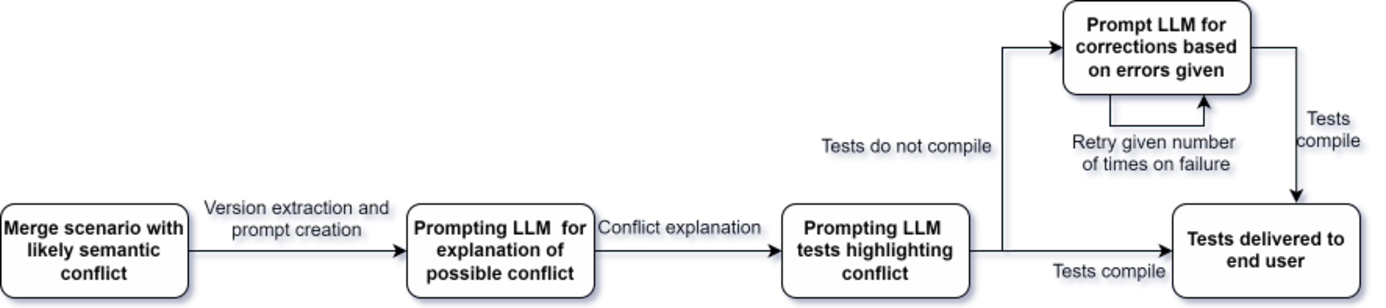
\includegraphics[width=1\linewidth]{figures/tool.pdf}
    \caption{Functioning pipeline of proposed tool.}
    \label{fig:tool}
\end{figure}

%%----------------------------------------
%% Final materials
%%----------------------------------------

%% Bibliography
%% Comment the next command if BibTeX file not used
%% bibliography is in ``myrefs.bib''
\PrintBib{myrefs}

%% 2021-07-20: change
%% comment next 2 commands if numbered appendices are not used
\appendix
\chapter{Extra stuff} \label{ap1:Lorem}

\section{Exploratory evaluation of ChatGPT's capabilities}

\subsection{Fabricated Examples}

In the initial step of work, we superficially explored ChatGPT's ability to generate tests for an example conflict of Point, where a distance method is altered from euclidean to manhattan in one branch and in the other branch, a move method is changed from using the value 1 for x and y movement to using the result of the distance calculation.

We tested two frameworks, first just asking for a test, with prompts based on the testing indications given by the DSL for the case:

\begin{itemize}
  \item A Dependency Based semantic conflict was possibly introduced in a 3-way merge. Develop a test for the class Point, that covers the methods move() and distance(), without calling distance() directly.
Before the merge, the class under test was: [base Point]
After the merge, it was: [merged Point].
  \item A Dependency Based semantic conflict was possibly introduced in a 3-way merge. Develop a test for the class Point, that covers the methods move() and distance(), without calling distance() directly.
Before the merge, the class under test was: [base Point]
In the branch A it was changed to: [A Point]
In the branch B it was changed to: [B Point]
After the merge, it was: [merged Point].

\end{itemize}

For this, the LLM simply took one version and created tests taking it as correct behaviour. In the first case, for Base and in the second for Merge. This is not ideal, as the first does not allow us to distinguish if the behaviour changed due to merging, or just do to changes in the branches. The latter takes merge as correct behaviour and will thus always fail.

Other tests involved first asking for an explanation if there was a merge conflict there, before asking for a test

\begin{itemize}
  \item We have done a merge on a piece of code.
Before the merge, the code was: [code]

In the branch A it was changed to: [code]

In the branch B it was changed to: [code]

After the merge it was: [code]

Do you believe there could be a merge conflict here? Where? Explain why.
  \item We have done a merge on a piece of code.
  
Before the merge, the code was: [code]

In the branch A it was changed to: [code]

In the branch B it was changed to: [code]

After the merge it was: [code]

Do you believe there could be a merge conflict here? Where? Explain why. Pay attention to both additions and modifications.
  \item We have done a merge on a piece of code code.
  
Before the merge, the code was: [code]

In the branch A it was changed to: [code]

In the branch B it was changed to: [code]

After the merge it was: [code]

Do you believe there could be a *semantic* merge conflict here? Where? Explain why. Pay attention to both additions and modifications.

\end{itemize}

The first two prompts failed. Indeed for prompt ChatGPT only mentioned the changes in move, but even after prompting it to pay attention to distance, it failed to identify the conflict. For both, it seemed to not understand what was being referred to when speaking of conflict, describing all changes as a "conflict". Thus it would say, there is a conflict between whether to use euclidian and manhattan distance and there is a conflict on how the move function works.

The last prompt given, highlighting the *semantic* aspect of the merge conflict, yielded good results, with the conflict being perfectly described, as seen in \Cref{fig:semconf}. After prompting for a test, it generates an appropriate one: it tests if the move function updates Point appropriately based on the euclidean distance. Thus it fails for base and branch B, where movement is still done with the value of 1, it passes for branch A as there move is based on distance; and it fails in merge, as now movement is being done with the distance calculation, but the calculation is now manhattan.

\begin{figure}
    \centering
    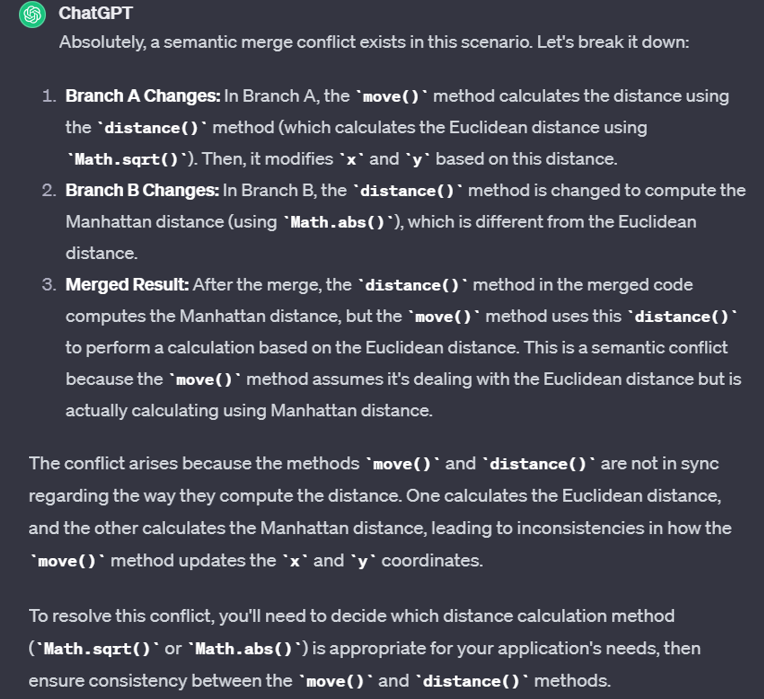
\includegraphics[width=0.75\linewidth]{figures/image.png}
    \caption{ChatGPT description of the semantic conflict}
    \label{fig:semconf}
\end{figure}

In simple fabricated scenarios, where simple conflicts were added to existing software solutions, ChatGPT showed ability to identify and describe the semantic conflict. Despite this, test generation remained complicated and few of the successful identification of semantic conflicts yielded working tests. The final prompt follows.

\begin{quote}
Generate a Junit unit test to identify this semantic conflict, knowing what you do now. The test must compile without errors and require no further alterations. It should require no further dependencies and import all classes correctly.
\end{quote}

While adapted to avoid common pitfalls, the tests generate still suffered from basic issues such as missing imports, which could be mitigated by prompting the LLM for correction automatically. More complex issues of implementation were present, such as calling the base function instead of dependent, wrong usage of construction and function returns, parameter types or unnecessary mocks. Further, when prompting for correction, the LLM often explains that the developer should correct this, thus further work needs to be done to ensure the tool does all the work itself.

\subsection{Real-World Merge Conflicts}

Prompting in real-world examples, or more complex fabricated examples, has produced far worse results. Several refinements were made to the prompts, most significantly: the usage of "git diff" to highlight the specific changes in branch A and branch B, the explanation of the conflict present and the specification of the target method where the conflict is evident. These modifications were largely unsuccessful and did not lead to identification of any significant amount conflicts.

We also had to reckon with size limits for messages. Thus, when necessary, we started with an explanatory prompt and then fed the information step by step. However, it remained crucial to remind the LLM of the goal in the last message.

\begin{quote}
We have done a merge on a piece of software and introduced a semantic conflict of types: "Update two different dependencies of a method or update one method and concurrently update one of its dependencies" and "Concurrent changes to the same method". I will now show the base commit, the diff in branch A, the diff in branch B, and the final merge version in 4 separate messages. At the end I want you to explain why and where the semantic conflict is present.
\end{quote}

Common issues are confusion between textual and semantic merges, which can be mitigated by clear explanation of what a semantic merge is; hallucinations of features not present in the code or hallucinations of changes where changes were not made; lack of focus on the methods where conflict is evident, despite reiterations; loss of focus when prompt has to be split into several messages. 
Rare close successes occured, particularly in cases where the conflict was asserted to be there in the prompt and could simply be described by explaining the changes made, such as parallel changes to collections initialization, as seen in \Cref{fig:cantfind}.

\begin{figure}
    \centering
    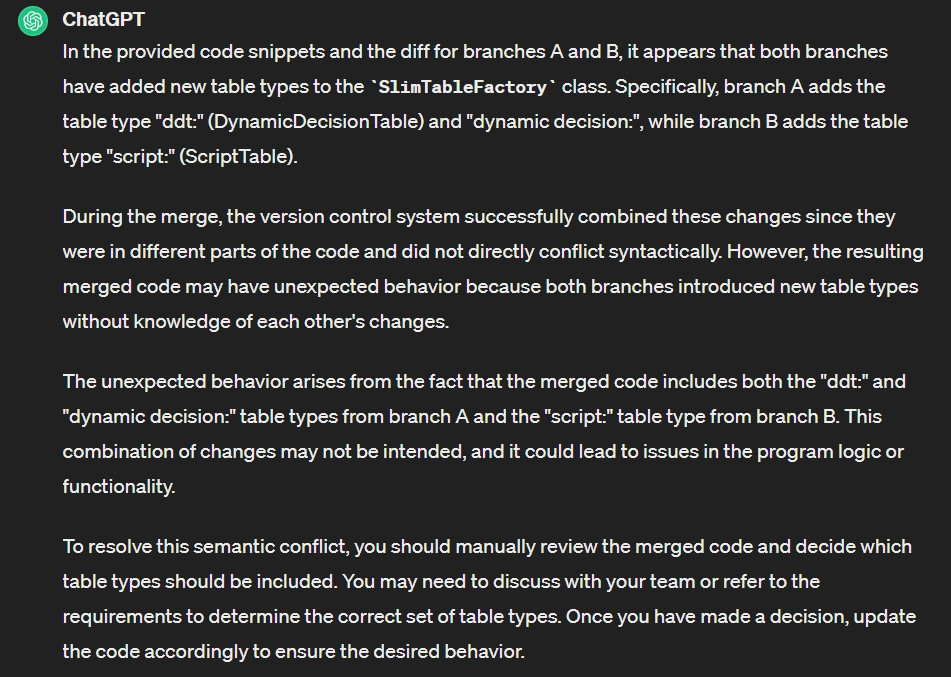
\includegraphics[width=1\linewidth]{figures/almostsemantic.jpg}
    \caption{ChatGPT describes the parallel changes as the origin of the conflict, but falls short of describing the emergent behaviour (in this case as simple as the different value returned by size())}
    \label{fig:cantfind}
\end{figure}

While we found that ChatGPT could not identify the semantic conflicts present in real software solutions, in some of \citet{kn:nuno}'s fabricated scenarios, these were correctly explained. Part of the difference between real-world examples and fabricated scenarios may come down to the information given. The fabricated scenarios were accompanied with a description of the specific semantic conflict present and the changes made perfectly reflected the description, with clear modifications and no extraneous changes. Thus it is possible collecting and offering that information with real-world scenarios may improve the ability of LLMs in this regard, but the higher "noise" of these scenarios may be too disruptive in this regard.

Another factor in consideration is the issue of dependencies, as so far testing had focused on just a unitary class. Given that semantic conflicts can involve interactions between classes and subclasses or other dependencies, it is relevant to provide further information. Initial tests just added one dependency, whether by calling a class methods or due to a inheritance relationship. An example, with the addition of an illustrative example of a semantic conflict follows.

\begin{quote}
We have done a merge on a piece of software and introduced a semantic conflict of type Parallel Changes in Method.

Semantic conflicts occur when concurrent and syntactic-correct changes in different regions of a source file or different files cause the software system to misbehave. For example, suppose there is a Java class `Point` with a method `distance()` that computes the Euclidean distance of a Point to the origin and Bob decides to modify `distance()` so it computes instead the Manhattan distance. At the same time, Alice, not aware of Bob's changes, creates a new method `move()` that uses `distance()` to calculate the Euclidean distance. Then, the changes of both developers are merged. As Bob and Alice did not modify the same lines of code, there is no textual conflict. There is neither a syntactic conflict as the merged code still compiles. However, the program now has an unexpected behaviour. The `move()` method introduced by Alice no longer moves a Point an Euclidean distance (as Alice was expecting) but rather moves a Manhattan distance

The affected declaration is copyWithDefaults().

A first message will detail the class before the merge, the diffs for both branches and the class after the merge. A second message will have a dependent class, whose methods indirectly call copyWithDefaults(). After I send these next two classes, identify and describe the semantic conflict.    
\end{quote}

A more complex evolution on this idea consisted of providing textual representations of UML graphs, such as plantUML call and structure graphs. These however proved to be complex in their own regard as they often induced the LLM to "forget" previous information and its goal, possibly due to their large size. A factor to consider, too, was that the information provided had to be limited in depth since, depending on the size of the software solution, a complete graph would be of extremely unwieldy size. Through some effort, we could get the LLM to recognize both the diagram and the class information, namely, by offering the diagram first.

\begin{quote}
We have done a merge on a piece of software. In this, we introduced a semantic conflict on the method dominates(State| State) of the class OpenTripPlanner. In a first message I will send a call diagram, in plantUML format. In a second message I will send the original class, the differences in the branches and the merged class.  At the end you must identify and explain the semantic conflict.
\end{quote}

However, it was particularly necessary to frequently refocus and concentrate the LLM. For example, after sending the diff and class information, reminding:

\begin{quote}
Explain why and where the semantic conflict is present, taking into account all the information provided in the last 2 messages. As mentioned before, focus on dominates(State| State). Make sure to mention information from the call diagram, if it is relevant to understanding the conflict.
\end{quote}

In the end, we were able to get the LLM to both recognize the merge information and the call diagram focused on the affected declaration and obtain a correct description of both the meaning of the diagram and the changes made in the merge. This however did not entail any improved description of the conflict, for all the cases tested.

Underscoring these experiments with real world test cases is an overlying issue: to properly identify a semantic conflict, we may have to analyze and take into account a large amount of data across several components of the software, while at the same time focusing on the specific components that were changed. While this is natural to a human, there is no clear way to select which information to feed and which to not in the LLM prompt: while a wider breadth of information may be necessary to identify the conflict, it is extremely likely to just induce further confusion and lead ChatGPT to focus on the wrong thing, or confuse different parts of code or even lose track of the task at hand as mentioned before.

\subsection{Test Generation without Conflict Understanding}

Given the difficulty of getting ChatGPT to provide accurate descriptions of the semantic conflicts, it was worth exploring whether the conflicts can be made evident just by generating tests targeting affected methods and classes. Several strategies were adopted: the prompting with the class after merge, the prompting with the class after merge and branch diffs and prompting with the class after merge and a structure graph. In most cases, where existing test suites where available, such information was also provided, with the prompt being reformulated to ask for its extension, rather than generation from scratch, as this shown to be important before~\cite{kn:githubcopilot}.

For 15 tests of 5 different projects, only 2 compiled, before and after prompting for corrections. One of these tested trivial additions to an array in both branches and the other identified a behaviour introduced in branch B that successfully carried over to merge, thus not a conflict. Positively, ChatGPT could understand the significance of this test working in branch B and merge but not A, as seen in \Cref{fig:testexplain}, suggesting it could understand the significance of a test failing for merge but not upper branches, which would indicate conflicts.

\begin{figure}
    \centering
    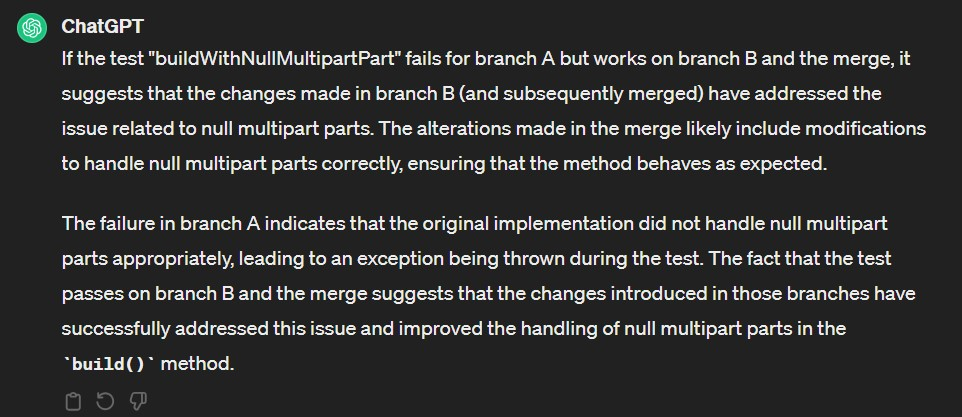
\includegraphics[width=1\linewidth]{figures/testexplain.jpg}
    \caption{ChatGPT explanation of meaning of failures and passes of test in different branches}
    \label{fig:testexplain}
\end{figure}

Common issues affecting test generation were:

\begin{itemize}
  \item Faulty importing/setup: Particularly relevant in the OKHttp case, the tool was patently unable to correctly call imports, just omitting them, even when expressly being given the package names and being told to import it.
  \item Invalid access: The LLM was generally unable to distinguish between private and public methods and frequently made attempts to invoke or access private methods and fields.
  \item Method/Field/Class Hallucination: ChatGPT frequently invoked non-existent methods, fields or even classes. In some classes this could also be related to matters of access, as it generated getter calls for private fields.
  \item Incomplete/Template Tests: Despite being prompted explicitly to generate complete tests that should compile, in several cases tests were generated with incomplete template helper methods and classes.
\end{itemize}

While feeding compilation error outputs could be a solution for these, in practice no test that failed to compile was fixed in this manner, as changes made did not fix or ignored the problems present. In some cases, while the logic of correction was sound logically, they were not helpful in the context of automatic test generation. For example, a "MockConverter" class was used in a test for the Retrofit project. Upon prompting for a fix, an import was added, which still naturally was non-functional. Upon prompting for another fix, ChatGPT provided a basic empty template for the MockConverter class. While a correctly implemented MockConverter class would fix the issue and allow the test to compile, the solution here would have been to drop the usage of the MockConverter class in the first place

Experiments were made to employ the usage of vector indexing to boost the capabilities of understanding code. The theory was that, by indexing the entire repository of code, we could proceed with prompting without having to decide which specific blocks of code should be required information in the prompt and that, during generation, the LLM could correctly identify the chain of dependencies, and which methods and parameters should be employed to properly test our desired methods. In this process we employed llama\_index, but the results fell short: due to an observed worse ability to generating code, focus was placed on the explanation of what should be done, with the prompting: "We want to create an extensive testing suite for the method [method] of the class [class]. How should we approach this? Which calls should we make, which parameters should we try and which results should be expected?"
Results were generic, many times not even referring to aspects of the code itself and still prone issues of hallucination, specifically the making of references to non-existent methods.

\section{Comparison of Developed Prompts with State of the Art}

To evaluated our progressively developed prompt with existing state of the art, we selected 5 prompts from comparison, henceforth referred as 1 \cite{kn:chattester}, 2 \cite{kn:siddiq2023empirical}, 3 \cite{kn:gptunitbra}, and 4 \cite{kn:chatunitest}. Our prompt, in turn, was 2-step prompt as follows:

\begin{quote}
The following class was altered in a merge, specifically the METHOD method. Analyse it and what it does, with focus on the method and its usage: CLASS INFO
\end{quote}

\begin{quote}
You are a Java developer. Due to changes in the METHOD method, you've been asked to write a complete test suite to identify possible errors introduced due to the changes. Write a junit test suite for the method. All classes must be correctly imported. The tests must compile without errors. The tests must be complete and require no modification and addition. No explanation needed.
\end{quote}

As subjects, we selected the basic fabricated Point class example, Antlr4, whose testing simply requires the length of a returned list and OkHttp, a more complex example requiring mocks and reflection for testing.
For each prompt, we generated 3 times and selected the best result for comparison.

For Point, we made the following observations:

Our prompt generated a suite with 3 tests, one of which had an incorrect assertion (A Point with coordinates -3,-4 was expected to move to 4,5 when it should move to 4,3). Despite this one wrong test, the correct ones successfully identified the conflict, as they tested manhattan distance movement. For an earlier branch, with euclidian distance movement, they would fail, showing the conflict.

Prompt 1 called the distance() method to identify where the Point should be and set assertions accordingly. While this tested the move method, it could not identify the conflict, as the assertions were dependent on the behaviour of distance(), as it changed so did they.

Prompt's 2,3,4 all made the same mistake: Starting from a point 3,4, they expected it to move to 7,8. As distance is 7, it should actually move to 10,11. Notably, Prompt 3 and 4 generated tests for distance and correctly identified it as 7.

For Antlr4, our prompt ran into errors: it could not correctly initialize the class, as the CodeGenerator object called by the constructor was incorrectly created. It also severely undercounted the number of keywords, leading to an incorrect assertion.
Prompt 1 showed improvement over ours, as it understood a null could be used in place of CodeGenerator, as it would not be used for our purposes. Despite this, it failed in the logic of the test, calling badWords unnecessarily: this is a private method that is already called by the getBadWords method we are testing. This same error was present in Prompt 2.
Prompt 3 generated nonsensical tests, just checking if the result of methods called was false. While it tested non-existent methods, it did not tested getBadWords as we desired.
Prompt 4 also called addBadWords despite not needing it, but as it was instructed to use Mockito, it avoided the error of calling a private method by using reflection. The rest of the test logic and the assertion was correct.


OkHttp should be the hardest to test, as the method under test and the method which calls it are private. The value returned (which we seek to test) is never publicly available.
Thus all prompts try and fail to call the private method. The exception is Prompt 3 which, by it's nature of generating for all methods rather than being told to generate for a specific one, avoids private methods. Surprisingly, Prompt 4 which had shown ability to use reflection in the previous subject, failed to produce a satisfactory result. Also of note is Prompt 2, which calls for 10 tests to be generated: in this case, to reach this 'quota', each parameter of the copied client was tested in a entirely different test, rather than just in a different assertion.
Despite failing, due to previously mentioned issue with access, Prompt 1 notably produced the best assertions, as it tested both functionalities of the method: the correct copying of defined parameters, and the returning of defaults for parameters that were not set.

\section{Selected Examples of RQ1 outputs}

\subsection{OkHttp, Trial 2}

\begin{prompt}
  You are a software developer that has to assess whether there is a semantic conflict in a merge commit.  Given the base version of the class, the diff from base to a version A, the diff from base to a version B and the merged version of the class, assess whether there is a semantic conflict and explain it.

Base version:
```java
/*
 * Copyright (C) 2012 Square, Inc.
 *
 * Licensed under the Apache License, Version 2.0 (the "License");
 * you may not use this file except in compliance with the License.
 * You may obtain a copy of the License at
 *
 *      http://www.apache.org/licenses/LICENSE-2.0
 *
 * Unless required by applicable law or agreed to in writing, software
 * distributed under the License is distributed on an "AS IS" BASIS,
 * WITHOUT WARRANTIES OR CONDITIONS OF ANY KIND, either express or implied.
 * See the License for the specific language governing permissions and
 * limitations under the License.
 */
package com.squareup.okhttp;

import com.squareup.okhttp.internal.http.HttpAuthenticator;
import com.squareup.okhttp.internal.http.HttpURLConnectionImpl;
import com.squareup.okhttp.internal.http.HttpsURLConnectionImpl;
import com.squareup.okhttp.internal.http.OkResponseCache;
import com.squareup.okhttp.internal.http.OkResponseCacheAdapter;
import java.net.CookieHandler;
import java.net.HttpURLConnection;
import java.net.Proxy;
import java.net.ProxySelector;
import java.net.ResponseCache;
import java.net.URL;
import java.util.Collections;
import java.util.LinkedHashSet;
import java.util.Set;
import javax.net.ssl.HostnameVerifier;
import javax.net.ssl.HttpsURLConnection;
import javax.net.ssl.SSLSocketFactory;

/** Configures and creates HTTP connections. */
public final class OkHttpClient {
  private Proxy proxy;
  private Set<Route> failedRoutes = Collections.synchronizedSet(new LinkedHashSet<Route>());
  private ProxySelector proxySelector;
  private CookieHandler cookieHandler;
  private ResponseCache responseCache;
  private SSLSocketFactory sslSocketFactory;
  private HostnameVerifier hostnameVerifier;
  private OkAuthenticator authenticator;
  private ConnectionPool connectionPool;
  private boolean followProtocolRedirects = true;

  /**
   * Sets the HTTP proxy that will be used by connections created by this
   * client. This takes precedence over {@link #setProxySelector}, which is
   * only honored when this proxy is null (which it is by default). To disable
   * proxy use completely, call {@code setProxy(Proxy.NO_PROXY)}.
   */
  public OkHttpClient setProxy(Proxy proxy) {
    this.proxy = proxy;
    return this;
  }

  public Proxy getProxy() {
    return proxy;
  }

  /**
   * Sets the proxy selection policy to be used if no {@link #setProxy proxy}
   * is specified explicitly. The proxy selector may return multiple proxies;
   * in that case they will be tried in sequence until a successful connection
   * is established.
   *
   * <p>If unset, the {@link ProxySelector#getDefault() system-wide default}
   * proxy selector will be used.
   */
  public OkHttpClient setProxySelector(ProxySelector proxySelector) {
    this.proxySelector = proxySelector;
    return this;
  }

  public ProxySelector getProxySelector() {
    return proxySelector;
  }

  /**
   * Sets the cookie handler to be used to read outgoing cookies and write
   * incoming cookies.
   *
   * <p>If unset, the {@link CookieHandler#getDefault() system-wide default}
   * cookie handler will be used.
   */
  public OkHttpClient setCookieHandler(CookieHandler cookieHandler) {
    this.cookieHandler = cookieHandler;
    return this;
  }

  public CookieHandler getCookieHandler() {
    return cookieHandler;
  }

  /**
   * Sets the response cache to be used to read and write cached responses.
   *
   * <p>If unset, the {@link ResponseCache#getDefault() system-wide default}
   * response cache will be used.
   */
  public OkHttpClient setResponseCache(ResponseCache responseCache) {
    this.responseCache = responseCache;
    return this;
  }

  public ResponseCache getResponseCache() {
    return responseCache;
  }

  private OkResponseCache okResponseCache() {
    if (responseCache instanceof HttpResponseCache) {
      return ((HttpResponseCache) responseCache).okResponseCache;
    } else if (responseCache != null) {
      return new OkResponseCacheAdapter(responseCache);
    } else {
      return null;
    }
  }

  /**
   * Sets the socket factory used to secure HTTPS connections.
   *
   * <p>If unset, the {@link HttpsURLConnection#getDefaultSSLSocketFactory()
   * system-wide default} SSL socket factory will be used.
   */
  public OkHttpClient setSSLSocketFactory(SSLSocketFactory sslSocketFactory) {
    this.sslSocketFactory = sslSocketFactory;
    return this;
  }

  public SSLSocketFactory getSslSocketFactory() {
    return sslSocketFactory;
  }

  /**
   * Sets the verifier used to confirm that response certificates apply to
   * requested hostnames for HTTPS connections.
   *
   * <p>If unset, the {@link HttpsURLConnection#getDefaultHostnameVerifier()
   * system-wide default} hostname verifier will be used.
   */
  public OkHttpClient setHostnameVerifier(HostnameVerifier hostnameVerifier) {
    this.hostnameVerifier = hostnameVerifier;
    return this;
  }

  public HostnameVerifier getHostnameVerifier() {
    return hostnameVerifier;
  }

  /**
   * Sets the authenticator used to respond to challenges from the remote web
   * server or proxy server.
   *
   * <p>If unset, the {@link Authenticator#setDefault system-wide default}
   * authenticator will be used.
   */
  public OkHttpClient setAuthenticator(OkAuthenticator authenticator) {
    this.authenticator = authenticator;
    return this;
  }

  public OkAuthenticator getAuthenticator() {
    return authenticator;
  }

  /**
   * Sets the connection pool used to recycle HTTP and HTTPS connections.
   *
   * <p>If unset, the {@link ConnectionPool#getDefault() system-wide
   * default} connection pool will be used.
   */
  public OkHttpClient setConnectionPool(ConnectionPool connectionPool) {
    this.connectionPool = connectionPool;
    return this;
  }

  public ConnectionPool getConnectionPool() {
    return connectionPool;
  }

  /**
   * Configure this client to follow redirects from HTTPS to HTTP and from HTTP
   * to HTTPS.
   *
   * <p>If unset, protocol redirects will be followed. This is different than
   * the built-in {@code HttpURLConnection}'s default.
   */
  public OkHttpClient setFollowProtocolRedirects(boolean followProtocolRedirects) {
    this.followProtocolRedirects = followProtocolRedirects;
    return this;
  }

  public boolean getFollowProtocolRedirects() {
    return followProtocolRedirects;
  }

  public HttpURLConnection open(URL url) {
    String protocol = url.getProtocol();
    OkHttpClient copy = copyWithDefaults();
    if (protocol.equals("http")) {
      return new HttpURLConnectionImpl(url, copy, copy.okResponseCache(), copy.failedRoutes);
    } else if (protocol.equals("https")) {
      return new HttpsURLConnectionImpl(url, copy, copy.okResponseCache(), copy.failedRoutes);
    } else {
      throw new IllegalArgumentException("Unexpected protocol: " + protocol);
    }
  }

  /**
   * Returns a shallow copy of this OkHttpClient that uses the system-wide default for
   * each field that hasn't been explicitly configured.
   */
  private OkHttpClient copyWithDefaults() {
    OkHttpClient result = new OkHttpClient();
    result.proxy = proxy;
    result.failedRoutes = failedRoutes;
    result.proxySelector = proxySelector != null ? proxySelector : ProxySelector.getDefault();
    result.cookieHandler = cookieHandler != null ? cookieHandler : CookieHandler.getDefault();
    result.responseCache = responseCache != null ? responseCache : ResponseCache.getDefault();
    result.sslSocketFactory = sslSocketFactory != null
        ? sslSocketFactory
        : HttpsURLConnection.getDefaultSSLSocketFactory();
    result.hostnameVerifier = hostnameVerifier != null
        ? hostnameVerifier
        : HttpsURLConnection.getDefaultHostnameVerifier();
    result.authenticator = authenticator != null
        ? authenticator
        : HttpAuthenticator.SYSTEM_DEFAULT;
    result.connectionPool = connectionPool != null ? connectionPool : ConnectionPool.getDefault();
    result.followProtocolRedirects = followProtocolRedirects;
    return result;
  }
}
```

Diff version A and the base:
```diff
@@ -15,6 +15,7 @@
  */
 package com.squareup.okhttp;

+import com.squareup.okhttp.internal.Util;
 import com.squareup.okhttp.internal.http.HttpAuthenticator;
 import com.squareup.okhttp.internal.http.HttpURLConnectionImpl;
 import com.squareup.okhttp.internal.http.HttpsURLConnectionImpl;
@@ -26,8 +27,10 @@ import java.net.Proxy;
 import java.net.ProxySelector;
 import java.net.ResponseCache;
 import java.net.URL;
+import java.util.Arrays;
 import java.util.Collections;
 import java.util.LinkedHashSet;
+import java.util.List;
 import java.util.Set;
 import javax.net.ssl.HostnameVerifier;
 import javax.net.ssl.HttpsURLConnection;
@@ -35,8 +38,12 @@ import javax.net.ssl.SSLSocketFactory;

 /** Configures and creates HTTP connections. */
 public final class OkHttpClient {
+  private static final List<String> DEFAULT_TRANSPORTS
+      = Util.immutableList(Arrays.asList("spdy/3", "http/1.1"));
+
   private Proxy proxy;
-  private Set<Route> failedRoutes = Collections.synchronizedSet(new LinkedHashSet<Route>());
+  private List<String> transports;
+  private final Set<Route> failedRoutes;
   private ProxySelector proxySelector;
   private CookieHandler cookieHandler;
   private ResponseCache responseCache;
@@ -46,6 +53,14 @@ public final class OkHttpClient {
   private ConnectionPool connectionPool;
   private boolean followProtocolRedirects = true;

+  public OkHttpClient() {
+    this.failedRoutes = Collections.synchronizedSet(new LinkedHashSet<Route>());
+  }
+
+  private OkHttpClient(OkHttpClient copyFrom) {
+    this.failedRoutes = copyFrom.failedRoutes; // Avoid allocating an unnecessary LinkedHashSet.
+  }
+
   /**
    * Sets the HTTP proxy that will be used by connections created by this
    * client. This takes precedence over {@link #setProxySelector}, which is
@@ -155,7 +170,7 @@ public final class OkHttpClient {
    * Sets the authenticator used to respond to challenges from the remote web
    * server or proxy server.
    *
-   * <p>If unset, the {@link Authenticator#setDefault system-wide default}
+   * <p>If unset, the {@link java.net.Authenticator#setDefault system-wide default}
    * authenticator will be used.
    */
   public OkHttpClient setAuthenticator(OkAuthenticator authenticator) {
@@ -198,6 +213,49 @@ public final class OkHttpClient {
     return followProtocolRedirects;
   }

+  /**
+   * Configure the transports used by this client to communicate with remote
+   * servers. By default this client will prefer the most efficient transport
+   * available, falling back to more ubiquitous transports. Applications should
+   * only call this method to avoid specific compatibility problems, such as web
+   * servers that behave incorrectly when SPDY is enabled.
+   *
+   * <p>The following transports are currently supported:
+   * <ul>
+   *   <li><a href="http://www.w3.org/Protocols/rfc2616/rfc2616.html">http/1.1</a>
+   *   <li><a href="http://www.chromium.org/spdy/spdy-protocol/spdy-protocol-draft3">spdy/3</a>
+   * </ul>
+   *
+   * <p><strong>This is an evolving set.</strong> Future releases may drop
+   * support for transitional transports (like spdy/3), in favor of their
+   * successors (spdy/4 or http/2.0). The http/1.1 transport will never be
+   * dropped.
+   *
+   * <p>If multiple protocols are specified, <a
+   * href="https://technotes.googlecode.com/git/nextprotoneg.html">NPN</a> will
+   * be used to negotiate a transport. Future releases may use another mechanism
+   * (such as <a href="http://tools.ietf.org/html/draft-friedl-tls-applayerprotoneg-02">ALPN</a>)
+   * to negotiate a transport.
+   *
+   * @param transports the transports to use, in order of preference. The list
+   *     must contain "http/1.1". It must not contain null.
+   */
+  public OkHttpClient setTransports(List<String> transports) {
+    transports = Util.immutableList(transports);
+    if (!transports.contains("http/1.1")) {
+      throw new IllegalArgumentException("transports doesn't contain http/1.1: " + transports);
+    }
+    if (transports.contains(null)) {
+      throw new IllegalArgumentException("transports must not contain null");
+    }
+    this.transports = transports;
+    return this;
+  }
+
+  public List<String> getTransports() {
+    return transports;
+  }
+
   public HttpURLConnection open(URL url) {
     String protocol = url.getProtocol();
     OkHttpClient copy = copyWithDefaults();
@@ -215,9 +273,8 @@ public final class OkHttpClient {
    * each field that hasn't been explicitly configured.
    */
   private OkHttpClient copyWithDefaults() {
-    OkHttpClient result = new OkHttpClient();
+    OkHttpClient result = new OkHttpClient(this);
     result.proxy = proxy;
-    result.failedRoutes = failedRoutes;
     result.proxySelector = proxySelector != null ? proxySelector : ProxySelector.getDefault();
     result.cookieHandler = cookieHandler != null ? cookieHandler : CookieHandler.getDefault();
     result.responseCache = responseCache != null ? responseCache : ResponseCache.getDefault();
@@ -232,6 +289,7 @@ public final class OkHttpClient {
         : HttpAuthenticator.SYSTEM_DEFAULT;
     result.connectionPool = connectionPool != null ? connectionPool : ConnectionPool.getDefault();
     result.followProtocolRedirects = followProtocolRedirects;
+    result.transports = transports != null ? transports : DEFAULT_TRANSPORTS;
     return result;
   }
 }
```

Diff version B and the base:
```diff
@@ -226,7 +227,7 @@ public final class OkHttpClient {
         : HttpsURLConnection.getDefaultSSLSocketFactory();
     result.hostnameVerifier = hostnameVerifier != null
         ? hostnameVerifier
-        : HttpsURLConnection.getDefaultHostnameVerifier();
+        : new OkHostnameVerifier();
     result.authenticator = authenticator != null
         ? authenticator
         : HttpAuthenticator.SYSTEM_DEFAULT;
```

Merge version:
```java
/*
 * Copyright (C) 2012 Square, Inc.
 *
 * Licensed under the Apache License, Version 2.0 (the "License");
 * you may not use this file except in compliance with the License.
 * You may obtain a copy of the License at
 *
 *      http://www.apache.org/licenses/LICENSE-2.0
 *
 * Unless required by applicable law or agreed to in writing, software
 * distributed under the License is distributed on an "AS IS" BASIS,
 * WITHOUT WARRANTIES OR CONDITIONS OF ANY KIND, either express or implied.
 * See the License for the specific language governing permissions and
 * limitations under the License.
 */
package com.squareup.okhttp;

import com.squareup.okhttp.internal.Util;
import com.squareup.okhttp.internal.http.HttpAuthenticator;
import com.squareup.okhttp.internal.http.HttpURLConnectionImpl;
import com.squareup.okhttp.internal.http.HttpsURLConnectionImpl;
import com.squareup.okhttp.internal.http.OkResponseCache;
import com.squareup.okhttp.internal.http.OkResponseCacheAdapter;
import com.squareup.okhttp.internal.tls.OkHostnameVerifier;
import java.net.CookieHandler;
import java.net.HttpURLConnection;
import java.net.Proxy;
import java.net.ProxySelector;
import java.net.ResponseCache;
import java.net.URL;
import java.util.Arrays;
import java.util.Collections;
import java.util.LinkedHashSet;
import java.util.List;
import java.util.Set;
import javax.net.ssl.HostnameVerifier;
import javax.net.ssl.HttpsURLConnection;
import javax.net.ssl.SSLSocketFactory;

/** Configures and creates HTTP connections. */
public final class OkHttpClient {
  private static final List<String> DEFAULT_TRANSPORTS
      = Util.immutableList(Arrays.asList("spdy/3", "http/1.1"));

  private Proxy proxy;
  private List<String> transports;
  private final Set<Route> failedRoutes;
  private ProxySelector proxySelector;
  private CookieHandler cookieHandler;
  private ResponseCache responseCache;
  private SSLSocketFactory sslSocketFactory;
  private HostnameVerifier hostnameVerifier;
  private OkAuthenticator authenticator;
  private ConnectionPool connectionPool;
  private boolean followProtocolRedirects = true;

  public OkHttpClient() {
    this.failedRoutes = Collections.synchronizedSet(new LinkedHashSet<Route>());
  }

  private OkHttpClient(OkHttpClient copyFrom) {
    this.failedRoutes = copyFrom.failedRoutes; // Avoid allocating an unnecessary LinkedHashSet.
  }

  /**
   * Sets the HTTP proxy that will be used by connections created by this
   * client. This takes precedence over {@link #setProxySelector}, which is
   * only honored when this proxy is null (which it is by default). To disable
   * proxy use completely, call {@code setProxy(Proxy.NO_PROXY)}.
   */
  public OkHttpClient setProxy(Proxy proxy) {
    this.proxy = proxy;
    return this;
  }

  public Proxy getProxy() {
    return proxy;
  }

  /**
   * Sets the proxy selection policy to be used if no {@link #setProxy proxy}
   * is specified explicitly. The proxy selector may return multiple proxies;
   * in that case they will be tried in sequence until a successful connection
   * is established.
   *
   * <p>If unset, the {@link ProxySelector#getDefault() system-wide default}
   * proxy selector will be used.
   */
  public OkHttpClient setProxySelector(ProxySelector proxySelector) {
    this.proxySelector = proxySelector;
    return this;
  }

  public ProxySelector getProxySelector() {
    return proxySelector;
  }

  /**
   * Sets the cookie handler to be used to read outgoing cookies and write
   * incoming cookies.
   *
   * <p>If unset, the {@link CookieHandler#getDefault() system-wide default}
   * cookie handler will be used.
   */
  public OkHttpClient setCookieHandler(CookieHandler cookieHandler) {
    this.cookieHandler = cookieHandler;
    return this;
  }

  public CookieHandler getCookieHandler() {
    return cookieHandler;
  }

  /**
   * Sets the response cache to be used to read and write cached responses.
   *
   * <p>If unset, the {@link ResponseCache#getDefault() system-wide default}
   * response cache will be used.
   */
  public OkHttpClient setResponseCache(ResponseCache responseCache) {
    this.responseCache = responseCache;
    return this;
  }

  public ResponseCache getResponseCache() {
    return responseCache;
  }

  private OkResponseCache okResponseCache() {
    if (responseCache instanceof HttpResponseCache) {
      return ((HttpResponseCache) responseCache).okResponseCache;
    } else if (responseCache != null) {
      return new OkResponseCacheAdapter(responseCache);
    } else {
      return null;
    }
  }

  /**
   * Sets the socket factory used to secure HTTPS connections.
   *
   * <p>If unset, the {@link HttpsURLConnection#getDefaultSSLSocketFactory()
   * system-wide default} SSL socket factory will be used.
   */
  public OkHttpClient setSSLSocketFactory(SSLSocketFactory sslSocketFactory) {
    this.sslSocketFactory = sslSocketFactory;
    return this;
  }

  public SSLSocketFactory getSslSocketFactory() {
    return sslSocketFactory;
  }

  /**
   * Sets the verifier used to confirm that response certificates apply to
   * requested hostnames for HTTPS connections.
   *
   * <p>If unset, the {@link HttpsURLConnection#getDefaultHostnameVerifier()
   * system-wide default} hostname verifier will be used.
   */
  public OkHttpClient setHostnameVerifier(HostnameVerifier hostnameVerifier) {
    this.hostnameVerifier = hostnameVerifier;
    return this;
  }

  public HostnameVerifier getHostnameVerifier() {
    return hostnameVerifier;
  }

  /**
   * Sets the authenticator used to respond to challenges from the remote web
   * server or proxy server.
   *
   * <p>If unset, the {@link java.net.Authenticator#setDefault system-wide default}
   * authenticator will be used.
   */
  public OkHttpClient setAuthenticator(OkAuthenticator authenticator) {
    this.authenticator = authenticator;
    return this;
  }

  public OkAuthenticator getAuthenticator() {
    return authenticator;
  }

  /**
   * Sets the connection pool used to recycle HTTP and HTTPS connections.
   *
   * <p>If unset, the {@link ConnectionPool#getDefault() system-wide
   * default} connection pool will be used.
   */
  public OkHttpClient setConnectionPool(ConnectionPool connectionPool) {
    this.connectionPool = connectionPool;
    return this;
  }

  public ConnectionPool getConnectionPool() {
    return connectionPool;
  }

  /**
   * Configure this client to follow redirects from HTTPS to HTTP and from HTTP
   * to HTTPS.
   *
   * <p>If unset, protocol redirects will be followed. This is different than
   * the built-in {@code HttpURLConnection}'s default.
   */
  public OkHttpClient setFollowProtocolRedirects(boolean followProtocolRedirects) {
    this.followProtocolRedirects = followProtocolRedirects;
    return this;
  }

  public boolean getFollowProtocolRedirects() {
    return followProtocolRedirects;
  }

  /**
   * Configure the transports used by this client to communicate with remote
   * servers. By default this client will prefer the most efficient transport
   * available, falling back to more ubiquitous transports. Applications should
   * only call this method to avoid specific compatibility problems, such as web
   * servers that behave incorrectly when SPDY is enabled.
   *
   * <p>The following transports are currently supported:
   * <ul>
   *   <li><a href="http://www.w3.org/Protocols/rfc2616/rfc2616.html">http/1.1</a>
   *   <li><a href="http://www.chromium.org/spdy/spdy-protocol/spdy-protocol-draft3">spdy/3</a>
   * </ul>
   *
   * <p><strong>This is an evolving set.</strong> Future releases may drop
   * support for transitional transports (like spdy/3), in favor of their
   * successors (spdy/4 or http/2.0). The http/1.1 transport will never be
   * dropped.
   *
   * <p>If multiple protocols are specified, <a
   * href="https://technotes.googlecode.com/git/nextprotoneg.html">NPN</a> will
   * be used to negotiate a transport. Future releases may use another mechanism
   * (such as <a href="http://tools.ietf.org/html/draft-friedl-tls-applayerprotoneg-02">ALPN</a>)
   * to negotiate a transport.
   *
   * @param transports the transports to use, in order of preference. The list
   *     must contain "http/1.1". It must not contain null.
   */
  public OkHttpClient setTransports(List<String> transports) {
    transports = Util.immutableList(transports);
    if (!transports.contains("http/1.1")) {
      throw new IllegalArgumentException("transports doesn't contain http/1.1: " + transports);
    }
    if (transports.contains(null)) {
      throw new IllegalArgumentException("transports must not contain null");
    }
    this.transports = transports;
    return this;
  }

  public List<String> getTransports() {
    return transports;
  }

  public HttpURLConnection open(URL url) {
    String protocol = url.getProtocol();
    OkHttpClient copy = copyWithDefaults();
    if (protocol.equals("http")) {
      return new HttpURLConnectionImpl(url, copy, copy.okResponseCache(), copy.failedRoutes);
    } else if (protocol.equals("https")) {
      return new HttpsURLConnectionImpl(url, copy, copy.okResponseCache(), copy.failedRoutes);
    } else {
      throw new IllegalArgumentException("Unexpected protocol: " + protocol);
    }
  }

  /**
   * Returns a shallow copy of this OkHttpClient that uses the system-wide default for
   * each field that hasn't been explicitly configured.
   */
  private OkHttpClient copyWithDefaults() {
    OkHttpClient result = new OkHttpClient(this);
    result.proxy = proxy;
    result.proxySelector = proxySelector != null ? proxySelector : ProxySelector.getDefault();
    result.cookieHandler = cookieHandler != null ? cookieHandler : CookieHandler.getDefault();
    result.responseCache = responseCache != null ? responseCache : ResponseCache.getDefault();
    result.sslSocketFactory = sslSocketFactory != null
        ? sslSocketFactory
        : HttpsURLConnection.getDefaultSSLSocketFactory();
    result.hostnameVerifier = hostnameVerifier != null
        ? hostnameVerifier
        : new OkHostnameVerifier();
    result.authenticator = authenticator != null
        ? authenticator
        : HttpAuthenticator.SYSTEM_DEFAULT;
    result.connectionPool = connectionPool != null ? connectionPool : ConnectionPool.getDefault();
    result.followProtocolRedirects = followProtocolRedirects;
    result.transports = transports != null ? transports : DEFAULT_TRANSPORTS;
    return result;
  }
}
```
\end{prompt}

\begin{response}
  To assess whether there is a semantic conflict in the merge commit, let's analyze the changes introduced in versions A and B and compare them to the base version, as well as examine the merged version.

  ### Changes in Version A:
  1. Added import statement: `import com.squareup.okhttp.internal.Util;`
  2. Added a new field `transports` of type `List<String>`.
  3. Modified the constructor to initialize `failedRoutes` using `Collections.synchronizedSet`.
  4. Added a new constructor that accepts an `OkHttpClient` instance to copy the `failedRoutes` set.
  5. Added setter and getter methods for the `transports` field.
  6. Modified the `copyWithDefaults()` method to include `transports`.
  
  ### Changes in Version B:
  1. Changed the default `hostnameVerifier` to `OkHostnameVerifier()` instead of using `HttpsURLConnection.getDefaultHostnameVerifier()`.
  
  ### Assessment of Semantic Conflict:
  There is a potential semantic conflict in the merge commit, specifically regarding the `hostnameVerifier` field.
  
  In Version A, the default `hostnameVerifier` is left unchanged. However, in Version B, the default `hostnameVerifier` is explicitly set to `OkHostnameVerifier()`.
  
  In the merge commit, the change from Version B is retained, and the default `hostnameVerifier` is set to `OkHostnameVerifier()`.
  
  ### Explanation:
  The conflict arises because both changes affect the same field (`hostnameVerifier`), but they prescribe different default values.
  
  In the merge commit, the decision was made to adopt the change from Version B, which explicitly sets the default `hostnameVerifier` to `OkHostnameVerifier()`. This decision potentially overrides any behavior or configuration related to the default `hostnameVerifier` set in Version A.
  
  If the intended behavior was to preserve the default `hostnameVerifier` as defined in Version A, then this would be considered a semantic conflict, as the behavior of the merged version may differ from the behavior of either Version A or Version B individually.
\end{response}

\subsection{Cart PF, Trial 1}

\begin{prompt}
  You are a software developer that has to assess whether there is a semantic conflict in a merge commit.  Given the base version of the class, the diff from base to a version A, the diff from base to a version B and the merged version of the class, assess whether there is a semantic conflict and explain it.

  Base version:
  ```java
  public class Cart {
      private List<Item> cartItems;
      private final User user;
  
      private static final Map<String, Double> discounts = Collections.unmodifiableMap(new HashMap<>() {{
          put("loyal", 0.1d); put("superpromo", 0.25d);
          put("30ff", 0.3d); put("2023", 0.3d);
          put("throwback", 0.15d); put("2024", 0.2d);
          put("fun", 0.05d); put("winner", 0.15d);
      }});
  
      public Set<String> getDiscountCodes() {
          return discounts.keySet();
      }
  
      public boolean checkForDiscountRenewal() {
          if(getDiscountCodes().size() <= 6)
              return true;
          else
              return false;
      }
  
  
      public Cart(User user) {
          this.user = user;
          cartItems = new ArrayList<>();
      }
  
      public double sum_items() {
          double sum = 0;
          for(Item item: cartItems) {
              sum += item.value*item.amount;
          }
          return Math.max(0, sum);
      }
      public double total_cost(double discount) {
          double sum = sum_items();
          return sum - sum * discount;
      }
  
      public void add_item(Item item) {
          cartItems.add(item);
      }
      public void checkout(String code) {
          double cost = total_cost(discounts.get(code));
          user.balance -= cost;
          cartItems.clear();
      }
  }
  ```
  
  Diff version A and the base:
  ```diff
  diff --git a/src/main/java/Cart.java b/src/main/java/Cart.java
  index cd65102..02b3420 100644
  --- a/src/main/java/Cart.java
  +++ b/src/main/java/Cart.java
  @@ -5,7 +5,7 @@ public class Cart {
       private final User user;
  
       private static final Map<String, Double> discounts = Collections.unmodifiableMap(new HashMap<>() {{
  -        put("loyal", 0.1d); put("superpromo", 0.25d);
  +        put("loyal", 0.1d);
           put("30ff", 0.3d); put("2023", 0.3d);
           put("throwback", 0.15d); put("2024", 0.2d);
           put("fun", 0.05d); put("winner", 0.15d);
  ```
  
  Diff version B and the base:
  ```diff
  diff --git a/src/main/java/Cart.java b/src/main/java/Cart.java
  index cd65102..509c220 100644
  --- a/src/main/java/Cart.java
  +++ b/src/main/java/Cart.java
  @@ -8,7 +8,7 @@ public class Cart {
           put("loyal", 0.1d); put("superpromo", 0.25d);
           put("30ff", 0.3d); put("2023", 0.3d);
           put("throwback", 0.15d); put("2024", 0.2d);
  -        put("fun", 0.05d); put("winner", 0.15d);
  +        put("fun", 0.05d);
       }});
  ```
  
  Merge version:
  ```java
  public class Cart {
      private List<Item> cartItems;
      private final User user;
  
      private static final Map<String, Double> discounts = Collections.unmodifiableMap(new HashMap<>() {{
          put("loyal", 0.1d);
          put("30ff", 0.3d); put("2023", 0.3d);
          put("throwback", 0.15d); put("2024", 0.2d);
          put("fun", 0.05d);
      }});
  
      public Set<String> getDiscountCodes() {
          return discounts.keySet();
      }
  
      public boolean checkForDiscountRenewal() {
          if(getDiscountCodes().size() <= 6)
              return true;
          else
              return false;
      }
  
  
      public Cart(User user) {
          this.user = user;
          cartItems = new ArrayList<>();
      }
  
      public double sum_items() {
          double sum = 0;
          for(Item item: cartItems) {
              sum += item.value*item.amount;
          }
          return Math.max(0, sum);
      }
      public double total_cost(double discount) {
          double sum = sum_items();
          return sum - sum * discount;
      }
  
      public void add_item(Item item) {
          cartItems.add(item);
      }
      public void checkout(String code) {
          double cost = total_cost(discounts.get(code));
          user.balance -= cost;
          cartItems.clear();
      }
  }
  ```
\end{prompt}

\begin{response}
  In this scenario, we're given the base version of a Java class `Cart`, along with two versions of changes (`A` and `B`) made to it, and finally, the merged version resulting from the merge of these two changes.

  Let's analyze the changes:
  
  1. **Diff Version A**:
     - It removes two discount codes, `"superpromo"` and `"winner"`.
     - This version retains 6 discount codes.
  
  2. **Diff Version B**:
     - It removes one discount code, `"winner"`.
     - This version also retains 6 discount codes.
  
  Now, let's look at the **Merge Version**:
     - It retains the changes from both diffs, removing discount codes `"superpromo"` and `"winner"`.
  
  Based on these changes, there isn't a semantic conflict in this merge. The changes from both versions `A` and `B` are independent and do not affect the same lines of code or properties. They both remove different discount codes, and the merge incorporates both of these changes correctly, resulting in a version that has those two discount codes removed.
  
  So, the merge is successful and preserves the intended changes from both versions without causing any conflicts in the functionality of the class.
\end{response}

\subsection{Antlr, Trial 1}

\begin{prompt}
  You are a software developer that has to assess whether there is a semantic conflict in a merge commit.  Given the base version of the class, the diff from base to a version A, the diff from base to a version B and the merged version of the class, assess whether there is a semantic conflict and explain it.

  Base version:
  ```java
  public class Python2Target extends Target {
    protected static final String[] python2Keywords = {
      "abs", "all", "any", "apply", "as",
      "bin", "bool", "buffer", "bytearray",
      "callable", "chr", "classmethod", "coerce", "compile", "complex",
      "delattr", "dict", "dir", "divmod",
      "enumerate", "eval", "execfile",
      "file", "filter", "float", "format", "frozenset",
      "getattr", "globals",
      "hasattr", "hash", "help", "hex",
      "id", "input", "int", "intern", "isinstance", "issubclass", "iter",
      "len", "list", "locals",
      "map", "max", "min", "next",
      "memoryview",
      "object", "oct", "open", "ord",
      "pow", "print", "property",
      "range", "raw_input", "reduce", "reload", "repr", "reversed", "round",
      "set", "setattr", "slice", "sorted", "staticmethod", "str", "sum", "super",
      "tuple", "type",
      "unichr", "unicode",
      "vars",
      "with",
      "xrange",
      "zip",
      "__import__",
      "True", "False", "None"
    };
  
    /** Avoid grammar symbols in this set to prevent conflicts in gen'd code. */
    protected final Set<String> badWords = new HashSet<String>();
  
    public Python2Target(CodeGenerator gen) {
      super(gen, "Python2");
    }
  
    @Override
    protected boolean visibleGrammarSymbolCausesIssueInGeneratedCode(GrammarAST idNode) {
      return getBadWords().contains(idNode.getText());
    }
  
    @Override
    protected STGroup loadTemplates() {
      STGroup result = super.loadTemplates();
      result.registerRenderer(String.class, new PythonStringRenderer(), true);
      return result;
    }
  
    protected static class PythonStringRenderer extends StringRenderer {
  
      @Override
      public String toString(Object o, String formatString, Locale locale) {
        return super.toString(o, formatString, locale);
      }
    }
  
    @Override
    public boolean wantsBaseListener() {
      return false;
    }
  
    @Override
    public boolean wantsBaseVisitor() {
      return false;
    }
  
    @Override
    public boolean supportsOverloadedMethods() {
      return false;
    }
  
    @Override
    public String getVersion() {
      return "4.5.2.1";
    }
  
    public Set<String> getBadWords() {
      if (badWords.isEmpty()) {
        addBadWords();
      }
  
      return badWords;
    }
  
    protected void addBadWords() {
      badWords.addAll(Arrays.asList(python2Keywords));
      badWords.add("rule");
      badWords.add("parserRule");
    }
  }
  ```
  
  Diff version A and the base:
  ```diff
  @@ -61,7 +61,7 @@ public class Python2Target extends Target {
                  "memoryview",
                  "object", "oct", "open", "ord",
                  "pow", "print", "property",
  -               "range", "raw_input", "reduce", "reload", "repr", "reversed", "round",
  +               "range", "raw_input", "reduce", "reload", "repr", "return", "reversed", "round",
                  "set", "setattr", "slice", "sorted", "staticmethod", "str", "sum", "super",
                  "tuple", "type",
                  "unichr", "unicode",
  ```
  
  Diff version B and the base:
  ```diff
  @@ -50,7 +50,7 @@ public class Python2Target extends Target {
                  "abs", "all", "any", "apply", "as",
                  "bin", "bool", "buffer", "bytearray",
                  "callable", "chr", "classmethod", "coerce", "compile", "complex",
  -               "delattr", "dict", "dir", "divmod",
  +               "del", "delattr", "dict", "dir", "divmod",
                  "enumerate", "eval", "execfile",
                  "file", "filter", "float", "format", "frozenset",
                  "getattr", "globals",
  ```
  
  Merge version:
  ```java
  public class Python2Target extends Target {
    protected static final String[] python2Keywords = {
      "abs", "all", "any", "apply", "as",
      "bin", "bool", "buffer", "bytearray",
      "callable", "chr", "classmethod", "coerce", "compile", "complex",
      "del", "delattr", "dict", "dir", "divmod",
      "enumerate", "eval", "execfile",
      "file", "filter", "float", "format", "frozenset",
      "getattr", "globals",
      "hasattr", "hash", "help", "hex",
      "id", "input", "int", "intern", "isinstance", "issubclass", "iter",
      "len", "list", "locals",
      "map", "max", "min", "next",
      "memoryview",
      "object", "oct", "open", "ord",
      "pow", "print", "property",
      "range", "raw_input", "reduce", "reload", "repr", "return", "reversed", "round",
      "set", "setattr", "slice", "sorted", "staticmethod", "str", "sum", "super",
      "tuple", "type",
      "unichr", "unicode",
      "vars",
      "with",
      "xrange",
      "zip",
      "__import__",
      "True", "False", "None"
    };
  
    /** Avoid grammar symbols in this set to prevent conflicts in gen'd code. */
    protected final Set<String> badWords = new HashSet<String>();
  
    public Python2Target(CodeGenerator gen) {
      super(gen, "Python2");
    }
  
    @Override
    protected boolean visibleGrammarSymbolCausesIssueInGeneratedCode(GrammarAST idNode) {
      return getBadWords().contains(idNode.getText());
    }
  
    @Override
    protected STGroup loadTemplates() {
      STGroup result = super.loadTemplates();
      result.registerRenderer(String.class, new PythonStringRenderer(), true);
      return result;
    }
  
    protected static class PythonStringRenderer extends StringRenderer {
  
      @Override
      public String toString(Object o, String formatString, Locale locale) {
        return super.toString(o, formatString, locale);
      }
    }
  
    @Override
    public boolean wantsBaseListener() {
      return false;
    }
  
    @Override
    public boolean wantsBaseVisitor() {
      return false;
    }
  
    @Override
    public boolean supportsOverloadedMethods() {
      return false;
    }
  
    @Override
    public String getVersion() {
      return "4.5.2.1";
    }
  
    public Set<String> getBadWords() {
      if (badWords.isEmpty()) {
        addBadWords();
      }
  
      return badWords;
    }
  
    protected void addBadWords() {
      badWords.addAll(Arrays.asList(python2Keywords));
      badWords.add("rule");
      badWords.add("parserRule");
    }
  }
  ```
\end{prompt}

\begin{response}
  In order to assess whether there's a semantic conflict in the merge commit, let's analyze the changes introduced in versions A and B compared to the base version, and then inspect the merged version.

  1. **Diff A vs Base:**
     - In version A, the `reduce` keyword was replaced with `return` in the `python2Keywords` array.
  
  2. **Diff B vs Base:**
     - In version B, the `del` keyword was added to the `python2Keywords` array.
  
  3. **Merged Version:**
     - The merged version includes both changes from versions A and B.
  
  Now, let's consider the semantic implications:
  
  - **Version A** replaces `reduce` with `return`. This change seems reasonable as `return` is a keyword used in functions to return values whereas `reduce` is a function for applying a function to all elements of an iterable.
    
  - **Version B** adds the `del` keyword. This is also sensible as `del` is used to delete objects.
  
  - **Merged Version** includes both changes, incorporating `return` from Version A and `del` from Version B.
  
  Upon examining the merged version, it appears there is no direct semantic conflict. Both changes are additions or replacements of Python keywords, and they don't interfere with each other. The `return` keyword addition and the `del` keyword addition are unrelated in terms of their functionality within Python.
  
  Thus, based on the provided information, there doesn't seem to be a semantic conflict in the merge commit. However, it's essential to perform thorough testing to ensure the correctness and compatibility of the merged code with the intended functionality.
\end{response}

\subsection{Fabricated RO, Trial 1}

\begin{prompt}
  You are a software developer that has to assess whether there is a semantic conflict in a merge commit.  Given the base version of the class, the diff from base to a version A, the diff from base to a version B and the merged version of the class, assess whether there is a semantic conflict and explain it.

  Base version:
  ```java
  package business;
  
  import java.io.Serializable;
  import java.util.List;
  import javax.persistence.*;
  import javax.persistence.DiscriminatorValue;
  
  /**
   * Entity implementation class for Entity: InstalacaoAssentos
   *
   */
  @Entity
  @DiscriminatorValue(value = "Assentos")
  public class InstalacaoAssentos extends Instalacao implements Serializable {
    
    private static final long serialVersionUID = 1L;
    
    @OneToMany
    private List<Lugar> lugares;
  
    public InstalacaoAssentos() {
      super();
    }
    
    @Override
    public List<Lugar> getLugares() {
      return lugares;
    }
  
    public void setLugares(List<Lugar> lugares) {
      this.lugares = lugares;
    }
  
    @Override
    public String getType() {
      return "TipoLugares.SENTADO";
    }
    
    @Override
    public int getOcupacao() {
      return lugares.size();
    }
  
    public String helpString(){
      StringBuilder result = new StringBuilder();
      result.append(super.toString());
      if(lugares != null)
        result.append(" | Lugares: " + lugares.size());
      else
        result.append(" | Lugares: null");
      return result.toString();
    }
     
  }
  ```
  
  Diff version A and the base:
  ```diff
  @@ -50,5 +50,9 @@ public class InstalacaoAssentos extends Instalacao implements Serializable {
                          result.append(" | Lugares: null");
                  return result.toString();
          }
  +
  +       public int hashString(){
  +               return helpString().hashCode();
  +       }
  
   }
  ```
  
  Diff version B and the base:
  ```diff
  @@ -40,15 +40,5 @@ public class InstalacaoAssentos extends Instalacao implements Serializable {
          public int getOcupacao() {
                  return lugares.size();
          }
  -
  -       public String helpString(){
  -               StringBuilder result = new StringBuilder();
  -               result.append(super.toString());
  -               if(lugares != null)
  -                       result.append(" | Lugares: " + lugares.size());
  -               else
  -                       result.append(" | Lugares: null");
  -               return result.toString();
  -       }
  
   }
  ```
  
  Merge version:
  ```java
  package business;
  
  import java.io.Serializable;
  import java.util.List;
  import javax.persistence.*;
  import javax.persistence.DiscriminatorValue;
  
  /**
   * Entity implementation class for Entity: InstalacaoAssentos
   *
   */
  @Entity
  @DiscriminatorValue(value = "Assentos")
  public class InstalacaoAssentos extends Instalacao implements Serializable {
    
    private static final long serialVersionUID = 1L;
    
    @OneToMany
    private List<Lugar> lugares;
  
    public InstalacaoAssentos() {
      super();
    }
    
    @Override
    public List<Lugar> getLugares() {
      return lugares;
    }
  
    public void setLugares(List<Lugar> lugares) {
      this.lugares = lugares;
    }
  
    @Override
    public String getType() {
      return "TipoLugares.SENTADO";
    }
    
    @Override
    public int getOcupacao() {
      return lugares.size();
    }
  
    public int hashString(){
      return helpString().hashCode();
    }
     
  }
  ```
\end{prompt}

\begin{response}
  Based on the provided information, let's analyze the changes made in versions A and B, and then compare them with the merge version to assess if there is a semantic conflict.

  In version A, the following changes were made:
  1. Added a method `hashString()` which computes the hash code of the string representation returned by the `helpString()` method.
  
  In version B, the following changes were made:
  1. Removed the `helpString()` method.
  
  Now, let's look at the merge version:
  - It retains the addition of the `hashString()` method from version A.
  - It removes the `helpString()` method as done in version B.
  
  There is a semantic conflict between the changes made in versions A and B:
  - Version A adds the `hashString()` method that relies on the `helpString()` method.
  - Version B removes the `helpString()` method which is used by `hashString()`.
  
  This results in a semantic conflict because the `hashString()` method in the merge version depends on the `helpString()` method which has been removed in version B. Therefore, if the `hashString()` method is invoked in the merge version, it will cause an error because the `helpString()` method is no longer available.
  
  To resolve this conflict, you may need to decide whether to keep the `hashString()` method and reintroduce the `helpString()` method or remove the `hashString()` method altogether, depending on the intended functionality of the merged class.
\end{response}
\section{Selected Examples of RQ2 outputs}

\subsection{Fabricated (OAC), Prompt 2, Trial 3}

\begin{prompt}
  You are a software developer that has to write a set of JUnit test cases to trigger a semantic conflict that has been identified in a merge commit. 
  Given the base version of the class, the diff from base to a version A, the diff from base to a version B and the merged version of the class, and an explanation of the existing semantic conflict, generate the appropriate JUnit test cases that trigger the conflict.
  
  Base version:
  ```java
  /**
   * 
   */
  package business.event;
  
  
  
  import java.time.LocalDate;
  import java.time.LocalTime;
  import java.util.ArrayList;
  import java.util.List;
  
  import javax.persistence.CascadeType;
  import javax.persistence.Column;
  import javax.persistence.Convert;
  import javax.persistence.Entity;
  import javax.persistence.EnumType;
  import javax.persistence.Enumerated;
  import javax.persistence.GeneratedValue;
  import javax.persistence.GenerationType;
  import javax.persistence.Id;
  import javax.persistence.ManyToOne;
  import javax.persistence.NamedQueries;
  import javax.persistence.NamedQuery;
  import javax.persistence.OneToMany;
  
  import business.util.Triplet;
  
  import business.producer.Producer;
  import business.ticket.Ticket;
  
  /**
   * 
   * An Event
   */
  @Entity
  @NamedQueries({
      @NamedQuery(name = Event.FIND_BY_NAME, query = "SELECT e FROM Event e WHERE e.name = :" + Event.STRING_NAME),
      @NamedQuery(name = Event.DATES_WITH_TICKETS_BY_STATE, query = "SELECT DISTINCT ed FROM SingleTicket t JOIN t.date ed WHERE ed.event.name = :"
          + Event.STRING_NAME + " AND ed.date > :" + Event.DATE_DATE
          + " AND t.state=:" + Event.ENUM_TICKET_STATE + " ORDER BY ed.date ASC"),
      @NamedQuery(name = Event.SEATS_FOR_EVENT_DATE_BY_STATE, query = "SELECT DISTINCT s FROM SingleTicket t JOIN t.date ed JOIN t.seat s WHERE ed.event.name = :"
          + Event.STRING_NAME + " AND ed.date = :" + Event.DATE_DATE
          + " AND t.state=:" + Event.ENUM_TICKET_STATE + " ORDER BY s.rowLetters ASC, s.seatNumber ASC"),
      @NamedQuery(name= Event._TICKETS, query= "SELECT e.tickets FROM Event e WHERE e.name = :" + Event.STRING_NAME),
      })
  
  public class Event {
  
    // Named query name constants
    public static final String FIND_BY_NAME = "Event.findByName";
    public static final String DATES_WITH_TICKETS_BY_STATE = "Event.datesWithTicketsByState";
    public static final String SEATS_FOR_EVENT_DATE_BY_STATE = "Event.seatsForEventDateByState";
    public static final String STRING_NAME = "name";
    public static final String DATE_DATE = "date";
    public static final String _TICKETS = "tickets";
    public static final String ENUM_TICKET_STATE = "ticket_state";
  
    /**
     * 
     */
    @Id @GeneratedValue(strategy = GenerationType.IDENTITY)
    private int id;
  
    /**
     * Event name
     */
    @Column(nullable = false, unique = true, name="Name")
    private String name;
  
    /**
     * the starting date when the tickets of the Event are available
     */
    @Convert(converter = LocalDateAttributeConverter.class)
    private LocalDate ticketStartSellingDate;
  
    /**
     * the type of the Event
     */
    @Enumerated(EnumType.STRING)
    private String type;
  
    /**
     * the dates of the Event
     */
    @OneToMany(mappedBy = "event", cascade = CascadeType.ALL, orphanRemoval = true)
    private List<EventDate> dates;
  
    /**
     * the tickets of the Event
     */
    @OneToMany(mappedBy = "event", cascade = CascadeType.ALL, orphanRemoval = true)
    private List<Ticket> tickets;
  
    /**
     * the venue where the Event will occur 
     */
    @ManyToOne
    private EventVenue venue;
  
    /**
     * the producer responsible for the Event
     */
    @ManyToOne
    private Producer producer;
  
  
    public Event() {
      this.dates = new ArrayList<>();
      this.tickets = new ArrayList<>();
    }
    
    /**
     * Constructor of the Event
     * @param producer producer of the event
     * @param eventType type of the Event
     * @param eventName name of the Event
     * @param eventDates dates of the Event
     */
    public Event(Producer producer, String eventType, String eventName, List<Triplet<LocalDate, LocalTime, LocalTime>> eventDates) {
  
  
      this.producer = producer;
      this.type = eventType;
      this.dates = new ArrayList<>();
      this.name = eventName;
      this.tickets = new ArrayList<>();
      for (Triplet<LocalDate, LocalTime, LocalTime> triple : eventDates) {
        dates.add(new EventDate(triple.getValue0(),triple.getValue1(),triple.getValue2(),this));
      }
    }
    
    
    // Getters and Setters
    
    public int getId() {
      return id;
    }
    
    /**
     * gets the starting date of the tickets
     * @return the starting date of the tickets
     */
    public LocalDate getStartSellingDate() {
      return ticketStartSellingDate;
    }
  
    /**
     * sets the starting date of the tickets
     * @param startSellingDate
     */
    public void setStartSellingDate(LocalDate startSellingDate) {
      this.ticketStartSellingDate = startSellingDate;
    }
    
    /**
     * gets the venue of the Event
     * @return the venue of the Event
     */
    public EventVenue getVenue() {
      return venue;
    }
    /**
     * sets the venue of the Event
     * @param venue of the event
     */
    public void setVenue(EventVenue venue) {
      this.venue = venue;
    }
    /**
     * gets the name of the Event
     * @return the name of the Event
     */
    public String getName() {
      return name;
    }
    /**
     * gets the type of the Event
     * @return the type of the Event
     */
    public String getType() {
      return type;
    }
    /**
     * get the tickets of the Event
     * @return the tickets
     */
    public List<Ticket> getTickets() {
      return tickets;
    }
    /**
     * gets the producer responsible of the Event
     * @return the producer of the Event
     */
    public Producer getProducer() {
      return producer;
    }
  
    public void setProducer(Producer p){
      producer = p;
    }
    
    /**
     * sets the tickets of the Event
     * @param tickets
     */
    public void setTickets(List<Ticket> tickets) {
      this.tickets = tickets;
    }
    
    /**
     * sets the name of the Event
     * @param name of the Event
     */
    public void setName(String name) {
      this.name = name;
    }
  
    /**
     * @return list of EventDate sorted by EventDate.date
     */
    public List<EventDate> getDates() {
      dates.sort(EventDate.ED_ASC);
      return dates;
    }
  }
  ```
  
  Diff version A and the base:
  ```diff
  @@ -95,7 +95,7 @@ public class Producer {
           *
           * @param resgistrationNumber
           */
  -       public void setResgistrationNumber(int resgistrationNumber) {
  +       private void setResgistrationNumber(int resgistrationNumber) {
                  this.registrationNumber = resgistrationNumber;
          }
          /**
  ```
  
  Diff version B and the base:
  ```diff
  @@ -199,6 +199,14 @@ public class Event {
          public void setProducer(Producer p){
                  producer = p;
          }
  +
  +       public int setProducerNumber(int n){
  +               if(producer != null){
  +                       producer.setResgistrationNumber(n);
  +                       return producer.getRegistrationNumber();
  +               }
  +               return -1;
  +       }
  
          /**
           * sets the tickets of the Event
  ```
  
  Merge version:
  ```java
  /**
   * 
   */
  package business.event;
  
  
  
  import java.time.LocalDate;
  import java.time.LocalTime;
  import java.util.ArrayList;
  import java.util.List;
  
  import javax.persistence.CascadeType;
  import javax.persistence.Column;
  import javax.persistence.Convert;
  import javax.persistence.Entity;
  import javax.persistence.EnumType;
  import javax.persistence.Enumerated;
  import javax.persistence.GeneratedValue;
  import javax.persistence.GenerationType;
  import javax.persistence.Id;
  import javax.persistence.ManyToOne;
  import javax.persistence.NamedQueries;
  import javax.persistence.NamedQuery;
  import javax.persistence.OneToMany;
  
  import business.util.Triplet;
  
  import business.producer.Producer;
  import business.ticket.Ticket;
  
  /**
   * 
   * An Event
   */
  @Entity
  @NamedQueries({
      @NamedQuery(name = Event.FIND_BY_NAME, query = "SELECT e FROM Event e WHERE e.name = :" + Event.STRING_NAME),
      @NamedQuery(name = Event.DATES_WITH_TICKETS_BY_STATE, query = "SELECT DISTINCT ed FROM SingleTicket t JOIN t.date ed WHERE ed.event.name = :"
          + Event.STRING_NAME + " AND ed.date > :" + Event.DATE_DATE
          + " AND t.state=:" + Event.ENUM_TICKET_STATE + " ORDER BY ed.date ASC"),
      @NamedQuery(name = Event.SEATS_FOR_EVENT_DATE_BY_STATE, query = "SELECT DISTINCT s FROM SingleTicket t JOIN t.date ed JOIN t.seat s WHERE ed.event.name = :"
          + Event.STRING_NAME + " AND ed.date = :" + Event.DATE_DATE
          + " AND t.state=:" + Event.ENUM_TICKET_STATE + " ORDER BY s.rowLetters ASC, s.seatNumber ASC"),
      @NamedQuery(name= Event._TICKETS, query= "SELECT e.tickets FROM Event e WHERE e.name = :" + Event.STRING_NAME),
      })
  
  public class Event {
  
    // Named query name constants
    public static final String FIND_BY_NAME = "Event.findByName";
    public static final String DATES_WITH_TICKETS_BY_STATE = "Event.datesWithTicketsByState";
    public static final String SEATS_FOR_EVENT_DATE_BY_STATE = "Event.seatsForEventDateByState";
    public static final String STRING_NAME = "name";
    public static final String DATE_DATE = "date";
    public static final String _TICKETS = "tickets";
    public static final String ENUM_TICKET_STATE = "ticket_state";
  
    /**
     * 
     */
    @Id @GeneratedValue(strategy = GenerationType.IDENTITY)
    private int id;
  
    /**
     * Event name
     */
    @Column(nullable = false, unique = true, name="Name")
    private String name;
  
    /**
     * the starting date when the tickets of the Event are available
     */
    @Convert(converter = LocalDateAttributeConverter.class)
    private LocalDate ticketStartSellingDate;
  
    /**
     * the type of the Event
     */
    @Enumerated(EnumType.STRING)
    private String type;
  
    /**
     * the dates of the Event
     */
    @OneToMany(mappedBy = "event", cascade = CascadeType.ALL, orphanRemoval = true)
    private List<EventDate> dates;
  
    /**
     * the tickets of the Event
     */
    @OneToMany(mappedBy = "event", cascade = CascadeType.ALL, orphanRemoval = true)
    private List<Ticket> tickets;
  
    /**
     * the venue where the Event will occur 
     */
    @ManyToOne
    private EventVenue venue;
  
    /**
     * the producer responsible for the Event
     */
    @ManyToOne
    private Producer producer;
  
  
    public Event() {
      this.dates = new ArrayList<>();
      this.tickets = new ArrayList<>();
    }
    
    /**
     * Constructor of the Event
     * @param producer producer of the event
     * @param eventType type of the Event
     * @param eventName name of the Event
     * @param eventDates dates of the Event
     */
    public Event(Producer producer, String eventType, String eventName, List<Triplet<LocalDate, LocalTime, LocalTime>> eventDates) {
  
  
      this.producer = producer;
      this.type = eventType;
      this.dates = new ArrayList<>();
      this.name = eventName;
      this.tickets = new ArrayList<>();
      for (Triplet<LocalDate, LocalTime, LocalTime> triple : eventDates) {
        dates.add(new EventDate(triple.getValue0(),triple.getValue1(),triple.getValue2(),this));
      }
    }
    
    
    // Getters and Setters
    
    public int getId() {
      return id;
    }
    
    /**
     * gets the starting date of the tickets
     * @return the starting date of the tickets
     */
    public LocalDate getStartSellingDate() {
      return ticketStartSellingDate;
    }
  
    /**
     * sets the starting date of the tickets
     * @param startSellingDate
     */
    public void setStartSellingDate(LocalDate startSellingDate) {
      this.ticketStartSellingDate = startSellingDate;
    }
    
    /**
     * gets the venue of the Event
     * @return the venue of the Event
     */
    public EventVenue getVenue() {
      return venue;
    }
    /**
     * sets the venue of the Event
     * @param venue of the event
     */
    public void setVenue(EventVenue venue) {
      this.venue = venue;
    }
    /**
     * gets the name of the Event
     * @return the name of the Event
     */
    public String getName() {
      return name;
    }
    /**
     * gets the type of the Event
     * @return the type of the Event
     */
    public String getType() {
      return type;
    }
    /**
     * get the tickets of the Event
     * @return the tickets
     */
    public List<Ticket> getTickets() {
      return tickets;
    }
    /**
     * gets the producer responsible of the Event
     * @return the producer of the Event
     */
    public Producer getProducer() {
      return producer;
    }
  
    public void setProducer(Producer p){
      producer = p;
    }
  
    public int setProducerNumber(int n){
      if(producer != null){
        producer.setResgistrationNumber(n);
        return producer.getRegistrationNumber();
      }
      return -1;
    }
    
    /**
     * sets the tickets of the Event
     * @param tickets
     */
    public void setTickets(List<Ticket> tickets) {
      this.tickets = tickets;
    }
    
    /**
     * sets the name of the Event
     * @param name of the Event
     */
    public void setName(String name) {
      this.name = name;
    }
  
    /**
     * @return list of EventDate sorted by EventDate.date
     */
    public List<EventDate> getDates() {
      dates.sort(EventDate.ED_ASC);
      return dates;
    }
  }
  ```
  
  Explanation of the semantic conflict: "In the provided scenario, let's analyze the changes made in versions A and B and then see if there's a semantic conflict in the merge commit.
  
  ### Version A Changes:
  1. The method `setResgistrationNumber(int resgistrationNumber)` in the `Producer` class was changed to `private`.
  
  ### Version B Changes:
  1. A new method `setProducerNumber(int n)` was added to the `Event` class, which sets the registration number of the producer.
     - This method internally calls `producer.setResgistrationNumber(n)`.
  
  ### Merge Commit:
  The merge commit contains changes from both versions A and B. It includes the changes in the `Producer` class from version A and the changes in the `Event` class from version B.
  
  ### Semantic Conflict Assessment:
  1. The change in version A made `setResgistrationNumber(int resgistrationNumber)` private in the `Producer` class.
  2. The change in version B introduced a new method `setProducerNumber(int n)` in the `Event` class, which attempts to set the registration number of the producer.
     - This new method internally tries to access `producer.setResgistrationNumber(n)`, which is now private due to the change in version A.
  
  ### Conclusion:
  There is a semantic conflict in the merge commit. The conflict arises because the `setProducerNumber(int n)` method in the `Event` class tries to access a method (`setResgistrationNumber(int resgistrationNumber)`) in the `Producer` class that has been made private in version A. As a result, this merge may lead to compilation errors or unexpected behavior in the application, as the method access is not allowed due to its visibility being changed to private. To resolve this conflict, you may need to modify either the visibility of the method in the `Producer` class or refactor the code in the `Event` class to not rely on this method directly."
  
  Generate just code with necessary imports. No explanation needed.
\end{prompt}

\begin{response}
```java
import business.event.Event;
import business.producer.Producer;
import org.junit.Test;
import static org.junit.Assert.*;

public class EventTest {

    @Test
    public void testSetProducerNumber() {
        Event event = new Event();
        Producer producer = new Producer();
        event.setProducer(producer);
        int registrationNumber = 12345;
        int result = event.setProducerNumber(registrationNumber);
        assertEquals(registrationNumber, result);
    }
}
```
\end{response}

\subsection{Point, Prompt 2, Trial 1}

\begin{prompt}
  You are a software developer that has to write a set of JUnit test cases to trigger a semantic conflict that has been identified in a merge commit. 
  Given the base version of the class, the diff from base to a version A, the diff from base to a version B and the merged version of the class, and an explanation of the existing semantic conflict, generate the appropriate JUnit test cases that trigger the conflict.
  
  Base version:
  ```java
  public class Point {
      private double x;
      private double y;
  
      public Point(double x, double y) {
          this.x = x;
          this.y = y;
      }
  
      public double getX() {
          return x;
      }
  
      public double getY() {
          return y;
      }
  
       public void move() {
           this.x += 1;
           this.y += 1;
       }
  
      public double distance() {
          return Math.sqrt(Math.pow(getX(), 2)+ Math.pow(getY(), 2));
      }
  
      public String toString() {
          return "(" + getX() + ", " + getY() + ")";
      }
  }
  ```
  
  Diff version A and the base:
  ```diff
  @@ -16,8 +16,9 @@ public class Point {
       }
  
        public void move() {
  -         this.x += 1;
  -         this.y += 1;
  +         double dist = distance();
  +         this.x += dist;
  +         this.y += dist;
        }
  
       public double distance() {
  ```
  
  Diff version B and the base:
  ```diff
  @@ -21,7 +21,7 @@ public class Point {
        }
  
       public double distance() {
  -        return Math.sqrt(Math.pow(getX(), 2)+ Math.pow(getY(), 2));
  +        return Math.abs(getX())+Math.abs(getY());
       }
  
       public String toString() {
  ```
  
  Merge version:
  ```java
  public class Point {
      private double x;
      private double y;
  
      public Point(double x, double y) {
          this.x = x;
          this.y = y;
      }
  
      public double getX() {
          return x;
      }
  
      public double getY() {
          return y;
      }
  
       public void move() {
           double dist = distance();
           this.x += dist;
           this.y += dist;
       }
  
      public double distance() {
          return Math.abs(getX())+Math.abs(getY());
      }
  
      public String toString() {
          return "(" + getX() + ", " + getY() + ")";
      }
  }
  ```
  
  Explanation of the semantic conflict: "To assess whether there is a semantic conflict in the merge commit, let's analyze the changes introduced in versions A and B compared to the base version, and then compare them with the merged version.
  
  ### Changes introduced in Version A:
  - The `move()` method has been modified to calculate the distance using the `distance()` method and then update the `x` and `y` coordinates accordingly.
  - This change effectively moves the point by the distance it currently is from the origin.
  
  ### Changes introduced in Version B:
  - The `distance()` method has been modified to calculate the Manhattan distance instead of the Euclidean distance.
  - The Manhattan distance is calculated by taking the absolute value of the x and y differences.
  
  ### Analysis of Merged Version:
  - The `move()` method from Version A has been kept in the merged version, which calculates the distance using the Euclidean distance.
  - The `distance()` method from Version B has been kept, which calculates the Manhattan distance.
  
  ### Potential Semantic Conflict:
  - The potential conflict arises from the inconsistency between how distance is calculated in the `move()` method and the `distance()` method in the merged version.
  - While the `move()` method assumes Euclidean distance for movement, the `distance()` method calculates the Manhattan distance.
  - This inconsistency could lead to unexpected behavior, as the `move()` method might not accurately reflect the intended behavior of the `distance()` method.
  
  ### Conclusion:
  - There is a semantic conflict in the merge commit because the merged version contains methods with conflicting assumptions about how distance should be calculated.
  - Resolving this conflict would require ensuring consistency in the distance calculation method used throughout the class, either sticking with Euclidean distance or Manhattan distance for both `move()` and `distance()` methods."
  
  Generate just code with necessary imports. No explanation needed.
\end{prompt}

\begin{response}
```java
import org.junit.Test;
import static org.junit.Assert.*;

public class PointTest {

    @Test
    public void testMove() {
        Point point = new Point(3, 4);
        point.move();
        assertEquals(7.0, point.getX(), 0.001);
        assertEquals(9.0, point.getY(), 0.001);
    }

    @Test
    public void testDistance() {
        Point point = new Point(3, 4);
        assertEquals(7.0, point.distance(), 0.001);
    }
}
```
\end{response}

\subsection{Cart (PF), Prompt 1, Trial 2}

\begin{prompt}
  You are a software developer that has to write a set of JUnit test cases to trigger a semantic conflict that has been identified in a merge commit. 
  Given the base version of the class, the diff from base to a version A, the diff from base to a version B and the merged version of the class, and an explanation of the existing semantic conflict, generate the appropriate JUnit test cases that trigger the conflict.
  
  Base version:
  ```java
  import java.util.Collections;
  import java.util.HashMap;
  import java.util.List;
  import java.util.Map;
  
  public class Cart {
      private List<Item> cartItems;
      private final User user;
  
      private static final Map<String, Double> discounts = Collections.unmodifiableMap(new HashMap<>() {{
          put("loyal", 0.1d);
          put("superpromo", 0.25d);
          put("30ff", 0.3d);
          put("2024", 0.2d);
      }});
  
  
      public Cart(User user) {
          this.user = user;
      }
  
      public double sum_items() {
          double sum = 0;
          for(Item item: cartItems) {
              sum += item.value*item.amount;
          }
          return Math.max(0, sum);
      }
      public double total_cost(double discount) {
          double sum = sum_items();
          return sum - sum * discount;
      }
  
      public void add_item(Item item) {
          cartItems.add(item);
      }
      public void checkout(String code) {
          double cost = total_cost(discounts.get(code));
          user.balance -= cost;
          cartItems.clear();
      }
  }
  ```
  
  Diff version A and the base:
  ```diff
  diff --git a/src/main/java/Cart.java b/src/main/java/Cart.java
  index 501b06f..e8e25b8 100644
  --- a/src/main/java/Cart.java
  +++ b/src/main/java/Cart.java
  @@ -12,6 +12,7 @@ public class Cart {
           put("superpromo", 0.25d);
           put("30ff", 0.3d);
           put("2024", 0.2d);
  +        put("megasaver", 0.4d);
       }});
  ```
  
  Diff version B and the base:
  ```diff
  diff --git a/src/main/java/Cart.java b/src/main/java/Cart.java
  index fbdd81f..0f8e11a 100644
  --- a/src/main/java/Cart.java
  +++ b/src/main/java/Cart.java
  @@ -9,7 +9,7 @@ public class Cart {
  
       private static final Map<String, Double> discounts = Collections.unmodifiableMap(new HashMap<>() {{
           put("loyal", 0.1d);
  -        put("superpromo", 0.25d);
  +        put("megasaver", 0.25d);
           put("30ff", 0.3d);
           put("2024", 0.2d);
       }});
  ```
  
  Merge version:
  ```java
  import java.util.Collections;
  import java.util.HashMap;
  import java.util.List;
  import java.util.Map;
  
  public class Cart {
      private List<Item> cartItems;
      private final User user;
  
      private static final Map<String, Double> discounts = Collections.unmodifiableMap(new HashMap<>() {{
          put("loyal", 0.1d);
          put("megasaver", 0.25d);
          put("30ff", 0.3d);
          put("2024", 0.2d);
          put("megasaver", 0.4d);
      }});
  
  
      public Cart(User user) {
          this.user = user;
      }
  
      public double sum_items() {
          double sum = 0;
          for(Item item: cartItems) {
              sum += item.value*item.amount;
          }
          return Math.max(0, sum);
      }
      public double total_cost(double discount) {
          double sum = sum_items();
          return sum - sum * discount;
      }
  
      public void add_item(Item item) {
          cartItems.add(item);
      }
      public void checkout(String code) {
          double cost = total_cost(discounts.get(code));
          user.balance -= cost;
          cartItems.clear();
      }
  }
  ```
  
  Explanation of the semantic conflict: In branch A, a discount with code megasaver is added, with value 0.4. In branch B, an existing discount with name superpromo and value 0.25 is renamed to megasaver. In the merge, this 0.25d is made useless, as the 0.4d discount replaces it when the list is created.
  Generate just code with necessary imports. No explanation needed.
\end{prompt}

\begin{response}
```java
import org.junit.jupiter.api.Test;
import static org.junit.jupiter.api.Assertions.*;

public class CartTest {

    @Test
    public void testMegaSaverDiscountConflict() {
        User user = new User();
        Cart cart = new Cart(user);
        Item item = new Item("Test", 10, 1);
        
        // Adding item to cart
        cart.add_item(item);
        
        // Checkout with megaSaver discount
        cart.checkout("megasaver");
        
        // Assert user balance after checkout
        assertEquals(user.balance, -6.0d);
    }
}
```
\end{response}

\subsection{Fabricated (RO), Trial 1}

\begin{prompt}
You are a software developer that has to write a set of JUnit test cases to trigger a semantic conflict that has been identified in a merge commit. 
Given the base version of the class, the diff from base to a version A, the diff from base to a version B and the merged version of the class, and an explanation of the existing semantic conflict, generate the appropriate JUnit test cases that trigger the conflict.

Base version:
```java
import java.util.Collections;
import java.util.HashMap;
import java.util.List;
import java.util.Map;

public class Cart {
    private List<Item> cartItems;
    private final User user;

    private static final Map<String, Double> discounts = Collections.unmodifiableMap(new HashMap<>() {{
        put("loyal", 0.1d);
        put("superpromo", 0.25d);
        put("30ff", 0.3d);
        put("2024", 0.2d);
    }});


    public Cart(User user) {
        this.user = user;
    }

    public double sum_items() {
        double sum = 0;
        for(Item item: cartItems) {
            sum += item.value*item.amount;
        }
        return Math.max(0, sum);
    }
    public double total_cost(double discount) {
        double sum = sum_items();
        return sum - sum * discount;
    }

    public void add_item(Item item) {
        cartItems.add(item);
    }
    public void checkout(String code) {
        double cost = total_cost(discounts.get(code));
        user.balance -= cost;
        cartItems.clear();
    }
}
```

Diff version A and the base:
```diff
diff --git a/src/main/java/Cart.java b/src/main/java/Cart.java
index fbdd81f..2846dd0 100644
--- a/src/main/java/Cart.java
+++ b/src/main/java/Cart.java
@@ -24,7 +24,7 @@ public class Cart {
          for(Item item: cartItems) {
              sum += item.value*item.amount;
          }
-        return Math.max(0, sum);
+        return sum;
      }
      public double total_cost(double discount) {
          double sum = sum_items();
```

Diff version B and the base:
```diff
diff --git a/src/main/java/Cart.java b/src/main/java/Cart.java
index fbdd81f..a90d713 100644
--- a/src/main/java/Cart.java
+++ b/src/main/java/Cart.java
@@ -22,7 +22,10 @@ public class Cart {
      public double sum_items() {
          double sum = 0;
          for(Item item: cartItems) {
-            sum += item.value*item.amount;
+            if(item.coupon)
+                sum -= item.value*item.amount;
+            else
+                sum += item.value*item.amount;
          }
          return Math.max(0, sum);
      }
diff --git a/src/main/java/Item.java b/src/main/java/Item.java
index 76a06c8..7b2db97 100644
--- a/src/main/java/Item.java
+++ b/src/main/java/Item.java
@@ -2,6 +2,7 @@ public class Item {

      public double value;
      public int amount;
+    public boolean coupon;

      public Item(int value) {
          this.value = value;
@@ -11,4 +12,14 @@ public class Item {
          this.value = value;
          this.amount = amount;
      }
+    public Item(int value, boolean coupon) {
+        this.value = value;
+        this.coupon = coupon;
+    }
+
+    public Item(int value, int amount, boolean coupon) {
+        this.value = value;
+        this.coupon = coupon;
+        this.amount = amount;
+    }
  }
```

Merge version:
```java
import java.util.Collections;
import java.util.HashMap;
import java.util.List;
import java.util.Map;

public class Cart {
    private List<Item> cartItems;
    private final User user;

    private static final Map<String, Double> discounts = Collections.unmodifiableMap(new HashMap<>() {{
        put("loyal", 0.1d);
        put("superpromo", 0.25d);
        put("30ff", 0.3d);
        put("2024", 0.2d);
    }});


    public Cart(User user) {
        this.user = user;
    }

    public double sum_items() {
        double sum = 0;
        for(Item item: cartItems) {
            if(item.coupon)
                sum -= item.value*item.amount;
            else
                sum += item.value*item.amount;
        }
        return sum;
    }
    public double total_cost(double discount) {
        double sum = sum_items();
        return sum - sum * discount;
    }

    public void add_item(Item item) {
        cartItems.add(item);
    }
    public void checkout(String code) {
        double cost = total_cost(discounts.get(code));
        user.balance -= cost;
        cartItems.clear();
    }
}
```
Explanation of the semantic conflict: A semantic conflicts because in branch A, a check ensuring that the sum of item values is 0 or more is removed. Simultaneously, in branch B, coupons are added, a type of item that is subtracted instead of summed. Because of both these changes, in the merge version it is possible to have the return of negative values, which is not intended.
Generate just code with necessary imports. No explanation needed.
\end{prompt}

\begin{response}
```java
import static org.junit.jupiter.api.Assertions.assertEquals;
import org.junit.jupiter.api.Test;

public class CartTest {

  @Test
  void testSumItemsWithCoupon() {
      Cart cart = new Cart(new User());
      cart.add_item(new Item(20, true));
      cart.add_item(new Item(30, true));
      assertEquals(-50, cart.sum_items());
  }

  @Test
  void testSumItemsWithoutCoupon() {
      Cart cart = new Cart(new User());
      cart.add_item(new Item(20));
      cart.add_item(new Item(30));
      assertEquals(50, cart.sum_items());
  }

  @Test
  void testTotalCostWithDiscount() {
      Cart cart = new Cart(new User());
      cart.add_item(new Item(20, true));
      cart.add_item(new Item(30, true));
      assertEquals(-30, cart.total_cost(0.1));
  }

  @Test
  void testTotalCostWithoutDiscount() {
      Cart cart = new Cart(new User());
      cart.add_item(new Item(20));
      cart.add_item(new Item(30));
      assertEquals(50, cart.total_cost(0.1));
  }
}
``` 
\end{response}
\section{Selected Examples of RQ3 outputs}

\subsection{Cart (PF), Prompt 1, Trial 1}

\begin{prompt}
  public class Cart {
    private List<Item> cartItems;
    private final User user;
    private static final Map<String, Double> discounts = Collections.unmodifiableMap(new HashMap<>() {{
        put("loyal", 0.1d);
        put("30ff", 0.3d); put("2023", 0.3d);
        put("throwback", 0.15d); put("2024", 0.2d);
        put("fun", 0.05d);
    }});
    public boolean checkForDiscountRenewal();
    public Cart(User);
    public double sum_items();
    public double total_cost(double);
    public void add_item(Item);
    public void checkout(String);
    //Focal Method
    public Set<String> getDiscountCodes() {
        return discounts.keySet();
    }
}
Please infer the intention of the "getDiscountCodes()"
\end{prompt}

\begin{answer}
The "getDiscountCodes()" method is intended to return a set of all available discount codes that can be applied to the items in the cart. This method allows the user to see the available discount codes and choose which one to apply during checkout.
\end{answer}

\begin{prompt}
The "getDiscountCodes()" method is intended to return a set of all available discount codes that can be applied to the items in the cart. This method allows the user to see the available discount codes and choose which one to apply during checkout.
You are a professional who writes Java test methods. Please write a test method for the "getDiscountCodes()" with the given Method intention.  
\end{prompt}

\begin{answer}
Sure, here is an example of a test method written in JUnit for the "getDiscountCodes()" method:

```java
import static org.junit.Assert.assertEquals;
import static org.junit.Assert.assertTrue;

import org.junit.Test;

public class CartTest {

    @Test
    public void testGetDiscountCodes() {
        Cart cart = new Cart(new User());
        
        Set<String> expectedDiscountCodes = new HashSet<>();
        expectedDiscountCodes.add("loyal");
        expectedDiscountCodes.add("30ff");
        expectedDiscountCodes.add("2023");
        expectedDiscountCodes.add("throwback");
        expectedDiscountCodes.add("2024");
        expectedDiscountCodes.add("fun");
        
        Set<String> actualDiscountCodes = cart.getDiscountCodes();
        
        assertEquals(expectedDiscountCodes.size(), actualDiscountCodes.size());
        for (String code : actualDiscountCodes) {
            assertTrue(expectedDiscountCodes.contains(code));
        }
    }
}
```

In this test method, a new instance of the `Cart` class is created and then the `getDiscountCodes()` method is called to retrieve the set of discount codes. The test method then compares the expected discount codes with the actual discount codes obtained from the `getDiscountCodes()` method. If they match, the test passes.  
\end{answer}

\subsection{Cart (PM), Prompt 1, Trial 1}

\begin{prompt}
  public class Cart {
    private List<Item> cartItems;
    private final User user;
    private static final Map<String, Double> discounts = Collections.unmodifiableMap(new HashMap<>() {{
        put("loyal", 0.1d);
        put("superpromo", 0.25d);
        put("30ff", 0.3d);
        put("2024", 0.2d);
    }});
    public Cart(User);
    public double sum_items();
    public double total_cost(double);
    public void add_item(Item);
    //Focal Method
    public void checkout(String code) {
        double cost = total_cost(discounts.get(code));
        if(cost==0)
            throw new RuntimeException("Cost can't be 0");
        user.balance -= cost;
        cartItems.clear();
    }
}
Please infer the intention of the "checkout(String)"
\end{prompt}

\begin{answer}
The intention of the "checkout(String)" method in the Cart class is to process the checkout of the items in the cart for a specific user with a given discount code. The method calculates the total cost of the items in the cart after applying the discount specified by the code, subtracts this cost from the user's balance, and then clears the cart items. If the cost after applying the discount is 0, it will throw a RuntimeException indicating that the cost cannot be 0.
\end{answer}

\begin{prompt}
The intention of the "checkout(String)" method in the Cart class is to process the checkout of the items in the cart for a specific user with a given discount code. The method calculates the total cost of the items in the cart after applying the discount specified by the code, subtracts this cost from the user's balance, and then clears the cart items. If the cost after applying the discount is 0, it will throw a RuntimeException indicating that the cost cannot be 0.
You are a professional who writes Java test methods. Please write a test method for the "checkout(String)" with the given Method intention.  
\end{prompt}

\begin{answer}
Sure, here is a test method for the "checkout(String)" method in the Cart class:

```java
import org.junit.jupiter.api.Test;
import static org.junit.jupiter.api.Assertions.*;

class CartTest {

    @Test
    void testCheckout_withValidDiscountCode() {
        User user = new User("John", 100.0);
        Cart cart = new Cart(user);
        Item item1 = new Item("Product1", 10.0);
        Item item2 = new Item("Product2", 20.0);
        cart.add_item(item1);
        cart.add_item(item2);

        cart.checkout("loyal");

        // Check user's balance after checkout
        assertEquals(69.0, user.balance);

        // Check cart is cleared after checkout
        assertTrue(cart.cartItems.isEmpty());
    }

    @Test
    void testCheckout_withZeroCostAfterDiscountCode() {
        User user = new User("Jane", 50.0);
        Cart cart = new Cart(user);
        Item item = new Item("Product", 40.0);
        cart.add_item(item);

        RuntimeException exception = assertThrows(RuntimeException.class, () -> {
            cart.checkout("superpromo");
        });

        assertEquals("Cost can't be 0", exception.getMessage());

        // Check user's balance is unchanged
        assertEquals(50.0, user.balance);

        // Check cart is not cleared
        assertFalse(cart.cartItems.isEmpty());
    }
}
\end{answer}

\subsection{Fabricated (OAC), Prompt 2}

\begin{prompt}
  //Event.java
  package business.event;
  
  
  
  import java.time.LocalDate;
  import java.time.LocalTime;
  import java.util.ArrayList;
  import java.util.List;
  
  import javax.persistence.CascadeType;
  import javax.persistence.Column;
  import javax.persistence.Convert;
  import javax.persistence.Entity;
  import javax.persistence.EnumType;
  import javax.persistence.Enumerated;
  import javax.persistence.GeneratedValue;
  import javax.persistence.GenerationType;
  import javax.persistence.Id;
  import javax.persistence.ManyToOne;
  import javax.persistence.NamedQueries;
  import javax.persistence.NamedQuery;
  import javax.persistence.OneToMany;
  
  import business.util.Triplet;
  
  import business.producer.Producer;
  import business.ticket.Ticket;
  
  /**
   * 
   * An Event
   */
  @Entity
  @NamedQueries({
      @NamedQuery(name = Event.FIND_BY_NAME, query = "SELECT e FROM Event e WHERE e.name = :" + Event.STRING_NAME),
      @NamedQuery(name = Event.DATES_WITH_TICKETS_BY_STATE, query = "SELECT DISTINCT ed FROM SingleTicket t JOIN t.date ed WHERE ed.event.name = :"
          + Event.STRING_NAME + " AND ed.date > :" + Event.DATE_DATE
          + " AND t.state=:" + Event.ENUM_TICKET_STATE + " ORDER BY ed.date ASC"),
      @NamedQuery(name = Event.SEATS_FOR_EVENT_DATE_BY_STATE, query = "SELECT DISTINCT s FROM SingleTicket t JOIN t.date ed JOIN t.seat s WHERE ed.event.name = :"
          + Event.STRING_NAME + " AND ed.date = :" + Event.DATE_DATE
          + " AND t.state=:" + Event.ENUM_TICKET_STATE + " ORDER BY s.rowLetters ASC, s.seatNumber ASC"),
      @NamedQuery(name= Event._TICKETS, query= "SELECT e.tickets FROM Event e WHERE e.name = :" + Event.STRING_NAME),
      })
  
  public class Event {
  
    // Named query name constants
    public static final String FIND_BY_NAME = "Event.findByName";
    public static final String DATES_WITH_TICKETS_BY_STATE = "Event.datesWithTicketsByState";
    public static final String SEATS_FOR_EVENT_DATE_BY_STATE = "Event.seatsForEventDateByState";
    public static final String STRING_NAME = "name";
    public static final String DATE_DATE = "date";
    public static final String _TICKETS = "tickets";
    public static final String ENUM_TICKET_STATE = "ticket_state";
  
    /**
     * 
     */
    @Id @GeneratedValue(strategy = GenerationType.IDENTITY)
    private int id;
  
    /**
     * Event name
     */
    @Column(nullable = false, unique = true, name="Name")
    private String name;
  
    /**
     * the starting date when the tickets of the Event are available
     */
    @Convert(converter = LocalDateAttributeConverter.class)
    private LocalDate ticketStartSellingDate;
  
    /**
     * the type of the Event
     */
    @Enumerated(EnumType.STRING)
    private String type;
  
    /**
     * the dates of the Event
     */
    @OneToMany(mappedBy = "event", cascade = CascadeType.ALL, orphanRemoval = true)
    private List<EventDate> dates;
  
    /**
     * the tickets of the Event
     */
    @OneToMany(mappedBy = "event", cascade = CascadeType.ALL, orphanRemoval = true)
    private List<Ticket> tickets;
  
    /**
     * the venue where the Event will occur 
     */
    @ManyToOne
    private EventVenue venue;
  
    /**
     * the producer responsible for the Event
     */
    @ManyToOne
    private Producer producer;
  
  
    public Event() {
      this.dates = new ArrayList<>();
      this.tickets = new ArrayList<>();
    }
    
    /**
     * Constructor of the Event
     * @param producer producer of the event
     * @param eventType type of the Event
     * @param eventName name of the Event
     * @param eventDates dates of the Event
     */
    public Event(Producer producer, String eventType, String eventName, List<Triplet<LocalDate, LocalTime, LocalTime>> eventDates) {
  
  
      this.producer = producer;
      this.type = eventType;
      this.dates = new ArrayList<>();
      this.name = eventName;
      this.tickets = new ArrayList<>();
      for (Triplet<LocalDate, LocalTime, LocalTime> triple : eventDates) {
        dates.add(new EventDate(triple.getValue0(),triple.getValue1(),triple.getValue2(),this));
      }
    }
    
    
    // Getters and Setters
    
    public int getId() {
      return id;
    }
    
    /**
     * gets the starting date of the tickets
     * @return the starting date of the tickets
     */
    public LocalDate getStartSellingDate() {
      return ticketStartSellingDate;
    }
  
    /**
     * sets the starting date of the tickets
     * @param startSellingDate
     */
    public void setStartSellingDate(LocalDate startSellingDate) {
      this.ticketStartSellingDate = startSellingDate;
    }
    
    /**
     * gets the venue of the Event
     * @return the venue of the Event
     */
    public EventVenue getVenue() {
      return venue;
    }
    /**
     * sets the venue of the Event
     * @param venue of the event
     */
    public void setVenue(EventVenue venue) {
      this.venue = venue;
    }
    /**
     * gets the name of the Event
     * @return the name of the Event
     */
    public String getName() {
      return name;
    }
    /**
     * gets the type of the Event
     * @return the type of the Event
     */
    public String getType() {
      return type;
    }
    /**
     * get the tickets of the Event
     * @return the tickets
     */
    public List<Ticket> getTickets() {
      return tickets;
    }
    /**
     * gets the producer responsible of the Event
     * @return the producer of the Event
     */
    public Producer getProducer() {
      return producer;
    }
  
    public void setProducer(Producer p){
      producer = p;
    }
  
    public int setProducerNumber(int n){
      if(producer != null){
        producer.setResgistrationNumber(n);
        return producer.getRegistrationNumber();
      }
      return -1;
    }
    
    /**
     * sets the tickets of the Event
     * @param tickets
     */
    public void setTickets(List<Ticket> tickets) {
      this.tickets = tickets;
    }
    
    /**
     * sets the name of the Event
     * @param name of the Event
     */
    public void setName(String name) {
      this.name = name;
    }
  
    /**
     * @return list of EventDate sorted by EventDate.date
     */
    public List<EventDate> getDates() {
      dates.sort(EventDate.ED_ASC);
      return dates;
    }
  }
  
  //EventTest.java
  package business.event;
  
  
  
  import java.time.LocalDate;
  import java.time.LocalTime;
  import java.util.ArrayList;
  import java.util.List;
  
  import javax.persistence.CascadeType;
  import javax.persistence.Column;
  import javax.persistence.Convert;
  import javax.persistence.Entity;
  import javax.persistence.EnumType;
  import javax.persistence.Enumerated;
  import javax.persistence.GeneratedValue;
  import javax.persistence.GenerationType;
  import javax.persistence.Id;
  import javax.persistence.ManyToOne;
  import javax.persistence.NamedQueries;
  import javax.persistence.NamedQuery;
  import javax.persistence.OneToMany;
  
  import business.util.Triplet;
  
  import business.producer.Producer;
  import business.ticket.Ticket;
  
  import org.junit.jupiter.api.Test;
  import static org.junit.jupiter.api.Assertions.*;
  
  
  /**
   * Test class of Event.
   * It contains 10 unit test cases for the
   * setProducerNumber(int) method.
   */
   class EventTest {
\end{prompt}

\begin{answer}
  public class EventTest {

  @Test
  void testSetProducerNumber_WhenProducerIsNull_ExpectNegativeOne() {
      Event event = new Event();
      int result = event.setProducerNumber(123);
      assertEquals(-1, result);
  }

  @Test
  void testSetProducerNumber_WhenProducerIsNotNull_ExpectProducerRegistrationNumber() {
      Producer producer = new Producer();
      Event event = new Event();
      event.setProducer(producer);
      int result = event.setProducerNumber(456);
      assertEquals(456, result);
  }

  @Test
  void testSetProducerNumber_WhenProducerIsNotNullAndRegistrationNumberIsAlreadySet_ExpectUpdatedProducerRegistrationNumber() {
      Producer producer = new Producer();
      producer.setRegistrationNumber(789);
      Event event = new Event();
      event.setProducer(producer);
      int result = event.setProducerNumber(101112);
      assertEquals(101112, result);
  }

  @Test
  void testSetProducerNumber_WhenProducerIsNotNullAndRegistrationNumberIsZero_ExpectUpdatedProducerRegistrationNumber() {
      Producer producer = new Producer();
      producer.setRegistrationNumber(0);
      Event event = new Event();
      event.setProducer(producer);
      int result = event.setProducerNumber(131415);
      assertEquals(131415, result);
  }

  @Test
  void testSetProducerNumber_WhenProducerIsNotNullAndRegistrationNumberIsNegative_ExpectUpdatedProducerRegistrationNumber() {
      Producer producer = new Producer();
      producer.setRegistrationNumber(-1);
      Event event = new Event();
      event.setProducer(producer);
      int result = event.setProducerNumber(161718);
      assertEquals(161718, result);
  }

  @Test
  void testSetProducerNumber_WhenProducerIsNotNullAndRegistrationNumberIsPositive_ExpectUpdatedProducerRegistrationNumber() {
      Producer producer = new Producer();
      producer.setRegistrationNumber(192021);
      Event event = new Event();
      event.setProducer(producer);
      int result = event.setProducerNumber(222324);
      assertEquals(222324, result);
  }

  @Test
  void testSetProducerNumber_WhenProducerIsNotNullAndRegistrationNumberIsMaxInt_ExpectUpdatedProducerRegistrationNumber() {
      Producer producer = new Producer();
      producer.setRegistrationNumber(Integer.MAX_VALUE);
      Event event = new Event();
      event.setProducer(producer);
      int result = event.setProducerNumber(123456);
      assertEquals(123456, result);
  }

  @Test
  void testSetProducerNumber_WhenProducerIsNotNullAndRegistrationNumberIsMinInt_ExpectUpdatedProducerRegistrationNumber() {
      Producer producer = new Producer();
      producer.setRegistrationNumber(Integer.MIN_VALUE);
      Event event = new Event();
      event.setProducer(producer);
      int result = event.setProducerNumber(7891011);
      assertEquals(7891011, result);
  }

  @Test
  void testSetProducerNumber_WhenProducerIsNotNullAndRegistrationNumberIsZero_ExpectZero() {
      Producer producer = new Producer();
      producer.setRegistrationNumber(0);
      Event event = new Event();
      event.setProducer(producer);
      int result = event.setProducerNumber(0);
      assertEquals(0, result);
  }

  @Test
  void testSetProducerNumber_WhenProducerIsNotNullAndRegistrationNumberIsNegative_ExpectNegativeNumber() {
      Producer producer = new Producer();
      producer.setRegistrationNumber(-123);
      Event event = new Event();
      event.setProducer(producer);
      int result = event.setProducerNumber(-456);
      assertEquals(-456, result);
  }
}
\end{answer}

\subsection{OkHttp, Prompt 3, Trial 1}

\begin{prompt}
  Please help me generate a whole JUnit test for a focal method in a focal class. I will provide the following information: 
  1. Required dependencies to import.
  2. The focal class signature.
  3. Source code of the focal method.
  4. Signatures of other methods and fields in the class.
  I need you to create a whole unit test using JUnit 4 and Mockito 3, ensuring optimal branch and line coverage. The test should include necessary imports for JUnit 4 andMockito 3, compile without errors, and use reflection to invoke private methods. No additional explanations required.
  
  The focal method is copyWithDefaults() in focal class OkHttpClient, the information is public final class OkHttpClient {
    private static final List<String> DEFAULT_TRANSPORTS
        = Util.immutableList(Arrays.asList("spdy/3", "http/1.1"));
    private Proxy proxy;
    private List<String> transports;
    private final Set<Route> failedRoutes;
    private ProxySelector proxySelector;
    private CookieHandler cookieHandler;
    private ResponseCache responseCache;
    private SSLSocketFactory sslSocketFactory;
    private HostnameVerifier hostnameVerifier;
    private OkAuthenticator authenticator;
    private ConnectionPool connectionPool;
    private boolean followProtocolRedirects = true;
    public OkHttpClient();
    private OkHttpClient(OkHttpClient);
    public OkHttpClient setProxy(Proxy);
    public Proxy getProxy();
    public OkHttpClient setProxySelector(ProxySelector);
    public ProxySelector getProxySelector();
    public OkHttpClient setCookieHandler(CookieHandler);
    public CookieHandler getCookieHandler();
    public OkHttpClient setResponseCache(ResponseCache);
    public ResponseCache getResponseCache();
    private OkResponseCache okResponseCache();
    public OkHttpClient setSSLSocketFactory(SSLSocketFactory);
    public SSLSocketFactory getSslSocketFactory();
    public OkHttpClient setHostnameVerifier(HostnameVerifier);
    public HostnameVerifier getHostnameVerifier();
    public OkHttpClient setAuthenticator(OkAuthenticator);
    public OkAuthenticator getAuthenticator();
    public OkHttpClient setConnectionPool(ConnectionPool);
    public ConnectionPool getConnectionPool();
    public OkHttpClient setFollowProtocolRedirects(boolean);
    public boolean getFollowProtocolRedirects();
    public OkHttpClient setTransports(List<String>);
    public List<String> getTransports();
    public HttpURLConnection open(URL);
    //Focal Method
    private OkHttpClient copyWithDefaults() {
      OkHttpClient result = new OkHttpClient(this);
      result.proxy = proxy;
      result.proxySelector = proxySelector != null ? proxySelector : ProxySelector.getDefault();
      result.cookieHandler = cookieHandler != null ? cookieHandler : CookieHandler.getDefault();
      result.responseCache = responseCache != null ? responseCache : ResponseCache.getDefault();
      result.sslSocketFactory = sslSocketFactory != null
          ? sslSocketFactory
          : HttpsURLConnection.getDefaultSSLSocketFactory();
      result.hostnameVerifier = hostnameVerifier != null
          ? hostnameVerifier
          : new OkHostnameVerifier();
      result.authenticator = authenticator != null
          ? authenticator
          : HttpAuthenticator.SYSTEM_DEFAULT;
      result.connectionPool = connectionPool != null ? connectionPool : ConnectionPool.getDefault();
      result.followProtocolRedirects = followProtocolRedirects;
      result.transports = transports != null ? transports : DEFAULT_TRANSPORTS;
      return result;
    }
  }
\end{prompt}

\begin{answer}
  import org.junit.Test;
import org.junit.runner.RunWith;
import org.mockito.Mockito;
import org.mockito.junit.MockitoJUnitRunner;

import java.net.Proxy;
import java.net.ProxySelector;
import java.net.ResponseCache;
import java.net.CookieHandler;
import java.net.URL;
import java.util.Arrays;
import java.util.List;

import javax.net.ssl.HostnameVerifier;
import javax.net.ssl.SSLSocketFactory;

import static org.junit.Assert.assertEquals;

@RunWith(MockitoJUnitRunner.class)
public class OkHttpClientTest {

    @Test
    public void testCopyWithDefaults() throws Exception {
        OkHttpClient okHttpClient = new OkHttpClient();
        OkHttpClient spyClient = Mockito.spy(okHttpClient);

        Proxy proxy = Mockito.mock(Proxy.class);
        ProxySelector proxySelector = Mockito.mock(ProxySelector.class);
        CookieHandler cookieHandler = Mockito.mock(CookieHandler.class);
        ResponseCache responseCache = Mockito.mock(ResponseCache.class);
        SSLSocketFactory sslSocketFactory = Mockito.mock(SSLSocketFactory.class);
        HostnameVerifier hostnameVerifier = Mockito.mock(HostnameVerifier.class);
        OkAuthenticator authenticator = Mockito.mock(OkAuthenticator.class);
        ConnectionPool connectionPool = Mockito.mock(ConnectionPool.class);

        List<String> transports = Arrays.asList("spdy/3", "http/1.1");

        Mockito.when(spyClient.getProxy()).thenReturn(proxy);
        Mockito.when(spyClient.getProxySelector()).thenReturn(proxySelector);
        Mockito.when(spyClient.getCookieHandler()).thenReturn(cookieHandler);
        Mockito.when(spyClient.getResponseCache()).thenReturn(responseCache);
        Mockito.when(spyClient.getSslSocketFactory()).thenReturn(sslSocketFactory);
        Mockito.when(spyClient.getHostnameVerifier()).thenReturn(hostnameVerifier);
        Mockito.when(spyClient.getAuthenticator()).thenReturn(authenticator);
        Mockito.when(spyClient.getConnectionPool()).thenReturn(connectionPool);
        Mockito.when(spyClient.getFollowProtocolRedirects()).thenReturn(true);
        Mockito.when(spyClient.getTransports()).thenReturn(transports);

        OkHttpClient result = spyClient.copyWithDefaults();

        assertEquals(proxy, result.getProxy());
        assertEquals(proxySelector != null ? proxySelector : ProxySelector.getDefault(), result.getProxySelector());
        assertEquals(cookieHandler != null ? cookieHandler : CookieHandler.getDefault(), result.getCookieHandler());
        assertEquals(responseCache != null ? responseCache : ResponseCache.getDefault(), result.getResponseCache());
        assertEquals(sslSocketFactory != null ? sslSocketFactory : HttpsURLConnection.getDefaultSSLSocketFactory(), result.getSslSocketFactory());
        assertEquals(hostnameVerifier != null ? hostnameVerifier : new OkHostnameVerifier(), result.getHostnameVerifier());
        assertEquals(authenticator != null ? authenticator : HttpAuthenticator.SYSTEM_DEFAULT, result.getAuthenticator());
        assertEquals(connectionPool != null ? connectionPool : ConnectionPool.getDefault(), result.getConnectionPool());
        assertEquals(true, result.getFollowProtocolRedirects());
        assertEquals(transports != null ? transports : OkHttpClient.DEFAULT_TRANSPORTS, result.getTransports());
    }
}
\end{answer}



%% Index
%% Uncomment next command if index is required
%% don't forget to run ``makeindex thesis'' command
% \PrintIndex

\end{document}
